\documentclass[a4paper]{article}

\newcommand{\mytitle}{Number Theory III}
\newcommand{\lecturer}{A. Bouganis}
\date{2020-2021}

\documentclass[a4paper, answers]{exam}

% tikzcd.yichuanshen.de/ tikcd diagrams
%======================%
%   Standard packages  %
%======================%
\usepackage[utf8]{inputenc}
\usepackage[T1]{fontenc}
\usepackage{lmodern}
\usepackage[UKenglish]{babel}
\usepackage{enumitem}
\usepackage{tasks}
\usepackage{graphicx}
\setlist[enumerate,1]{
  label={(\roman*)}
}
\usepackage{parskip}
\usepackage{hyperref}

%======================%
%        Maths         %
%======================%
\usepackage{amsfonts, mathtools, amsthm, amssymb}
\usepackage{xfrac}
\usepackage{bm}
\newcommand\N{\ensuremath{\mathbb{N}}}
\newcommand\R{\ensuremath{\mathbb{R}}}
\newcommand\Z{\ensuremath{\mathbb{Z}}}
\newcommand\Q{\ensuremath{\mathbb{Q}}}
\newcommand\C{\ensuremath{\mathbb{C}}}
\newcommand\F{\ensuremath{\mathbb{F}}}
\newcommand{\abs}[1]{\ensuremath{\left\lvert #1 \right\rvert}}
\newcommand\given[1][]{\:#1\vert\:}
\newcommand\restr[2]{{% we make the whole thing an ordinary symbol
  \left.\kern-\nulldelimiterspace % automatically resize the bar with \right
  #1 % the function
  \vphantom{\big|} % pretend it's a little taller at normal size
  \right|_{#2} % this is the delimiter
}}

\newcommand\corestr[2]{{% we make the whole thing an ordinary symbol
  \left.\kern-\nulldelimiterspace % automatically resize the bar with \right
  #1 % the function
  \vphantom{\big|} % pretend it's a little taller at normal size
  \right|^{#2} % this is the delimiter
}}
\usepackage{siunitx}

\usepackage{afterpage}

\usepackage{tikz-cd}
\usepackage{adjustbox}
\DeclareMathOperator{\norm}{N}
\DeclareMathOperator{\trace}{Tr}
\DeclareMathOperator*{\argmax}{arg\,max}
\DeclareMathOperator*{\argmin}{arg\,min}
\DeclareMathOperator*{\esssup}{ess\,sup}
\DeclareMathOperator*{\SL}{SL}
\DeclareMathOperator*{\GL}{GL}
\DeclareMathOperator*{\SO}{SO}
\DeclareMathOperator*{\aut}{Aut}
\DeclareMathOperator*{\id}{id}
\DeclareMathOperator*{\coker}{coker}
\DeclareMathOperator*{\im}{im}



%======================%
%       CompSci        %
%======================%
\usepackage{forest}
\usepackage{textgreek}
\usepackage{algpseudocode}

%======================%
%    Pretty tables     %
%======================%
\usepackage{booktabs}
\usepackage{caption}

\begin{document}
    \maketitle
    \tableofcontents
    \chapter{Asymptotic notation}
\lecture{1}{14/10}

Asymptotic notation is assumed knowledge from previous modules, 
this chapter serves as a brief recap. 
Let's start with some definitions.

\section{Problems and algorithms}

\begin{definition}[Algorithm]
    An \textbf{algorithm} is a program that accepts inputs and produce outputs.
\end{definition}

We call an algorithm \textbf{correct} if it halts with the correct output.

We use algorithm to solve \textbf{problems}. 
A \textbf{problem} can be thought of as a relationship between the inputs and outputs of an algorithm.

\begin{example}[Sorting]
    Here we introduce the widely studied \textbf{sorting problem}. 
    Let our input be a $n$-tuple $(a_1, a_2, \ldots, a_n)$. 
    The output to our algorithm should be the tuple 
    $(a_{i_1}, a_{i_2}, \ldots, a_{i_n})$ 
    where $(i_1, i_2, \ldots, i_n)$ is a reordering of $(1, 2, \ldots, n)$ such that 
    \[ a_{i_1} \leq a_{i_2} \leq \ldots \leq a_{i_n}. \]

    There are many examples of sorting algorithms that we have already studied:
    \begin{enumerate}
        \item insertion sort;
        \item merge sort; and
        \item meap sort.
    \end{enumerate}
\end{example}

Now that we know what problems and algorithms are, let's reintrouce asymptotic notation.

\section{Big-$O$ and friends}

\begin{definition}[Big-$O$]
    Let $f(n), g(n) \geq 0$. 
    We define big-$O$ of $g(n)$ as 
    \[ O(g(n)) = 
        \{
        f(n) : \;\exists\; k > 0 \; \exists \; N \in \N \;\forall\; n > N : 
        \lvert f(n) \rvert \leq k g(n)
        \}.
    \] 
    We mathematically describe this by saying that 
    $\lvert f(n) \rvert$ 
    is bounded above by $g(n)$ up to a constant factor asymptotically. 
    We can also define big-$O$ using the following limits definition: 
    \[ f(n) \in O(g(n)) \iff 
        \limsup_{n\to\infty} \left(\frac{\lvert f(n) \rvert}{g(n)}\right) < \infty; 
    \] 
    however, note that big-$O$ can not be rigorously defined using limits.
\end{definition}

You will most likely see the notation $f(n) = O(g(n))$ in literature (and this course!). 
This is a convention to mean $f(n) \in O(g(n))$.

\begin{definition}[Big-$\Omega$]
    Similarly, let $f(n), g(n) \geq 0$. 
    Then 
    \[\Omega(g(n)) = \{ f(n) : \;\exists\; k > 0 \;\exists\; N \in \N \;\forall\; n > N : f(n) \geq k g(n) \}.\] 
    Here we say that $f$ is bounded below by $g$ asymptotically.
\end{definition}

As a very loose analogy, we can look at Big-$O$ as representing the relation $\leq$. 
So 
$f(n) = O(g(n))$ 
is a similar relation for functions $f, g$ to the relation $a \leq b$ for $a, b \in \R$. 
Similarly, we can see big-$\Omega$ as representing the $\geq$ relation.

\begin{definition}[Big-$\Theta$]
    Let $f(n), g(n) \geq 0$. 
    Then 
    \[ \Theta(g(n)) = \{ f(n) : f(n) \in O(g(n)) \;\text{and}\; f(n) \in \Omega(g(n)) \}. \] 
    An alternative definition is 
    \[ \Theta(g(n)) = \{ f(n) : f(n) \in O(g(n)) \;\text{and}\; g(n) \in O(f(n)). \]
\end{definition}

\begin{proposition}
    Let $f(n), g(n) \geq 0$.
    \begin{enumerate}
        \item $f(n) = \Theta(g(n)) \iff g(n) = \Theta(f(n))$; and
        \item $f(n) = O(g(n)) \iff g(n) = \Omega(f(n))$.
    \end{enumerate}
\end{proposition}

\section{Little-$o$ and friends}

Following our analogy from earlier, 
we can see little-$o$ and little-$\omega$ for functions as the $<$ and $>$ relations for $\R$.

\begin{definition}[Little-$o$]
    We define little-$o$ of a function $g(n)$ to be 
    \[ o(g(n)) = 
        \{ f(n) : 
            \;\forall\; k > 0 \;\exists\; N \in \N : 
            kg(n) \leq f(n) \;\forall\; n > N 
        \}.
    \]
\end{definition}

\begin{definition}[Little-$\omega$]
    We define little-$\omega$ of a function $g(n)$ to be 
    \[ \omega(g(n) = \{ f(n) : 
        \;\forall\; k > 0 \;\exists\; N \in \N : f(n) \leq kg(n) \;\forall\; n > N 
        \}. 
    \]
\end{definition}

\begin{proposition}
    \begin{enumerate}
        \item $f(n) = o(g(n)) \iff g(n) = \omega(f(n))$;
        \item $f(n) = O(g(n)) \iff (f(n) = \Theta(g(n)) \;\text{or}\; (f(n) = o(g(n))$; and
        \item $f(n) = \Omega(g(n)) \iff (f(n) = \Theta(g(n)) \;\text{or}\; (f(n) = \omega(g(n))$.
    \end{enumerate}
\end{proposition}

Hopefully the last two points of the above proposition helps cements the analogy between asymptotic behaviour for functions and the $>$, $<$, $\leq$, and $\geq$ relations for $\R$.

\section{Running time}

\begin{definition}[Running time]
    Let $\alpha$ be some algorithm that takes an input $I$. 
    Then we define $T(I)$ as the time taken until $\alpha$ halts. 
    We define the \textbf{worst-case running time} as 
    \[ T(n) = \max{\{T(I) : \lvert I \rvert = n\}}, \] 
    here we denote the size of $I$ as $\lvert I \rvert$.
\end{definition}

This pretty much includes the entire recap for this module, 
but there is a comment to be made on asymptotic notation. 
When we look at the asymptotic behaviour of time complexity of some algorithm we do lose some information. 
Constants can have a large effect on the running time of an algorithm for small $n$, 
and we don't necessarily always run an algorithm for large $n$. 
It is important to understand the limiting behaviour of time complexity as well though. 

    \lecture{2}{10/10}

A note on notation, we may use $S^\star$ to denote a finite length tuple containing only elements in $S$. This is not the same as the complex analysis definition where $\C^\star = \C \setminus \{0\}$. For example, $(0, 0, 1, 1, 0 ,1) \in \{ 0, 1 \}^\star$.

\begin{definition}[]
    A language $\mathcal L$ is \textbf{Turing-Recognisable} if there exists a turing machine $\mathcal M$ that recognises it. That is, $\mathcal L = L(\mathcal M)$.
\end{definition}

\begin{definition}[]
    A language $\mathcal L$ is \textbf{Turing-Decideable} if there exists a turing machine $\mathcal M$ that accepts all $w \in \mathcal L$ and rejects all $w \not \in \mathcal L$.
\end{definition}

So we say that $\mathcal M$ recognises $\mathcal L$ if it accepts every word in $\mathcal L$, but $\mathcal M$ decides $\mathcal L$ if it accepts every word and rejects every word not in $\mathcal L$.

You may see the terminology `r.e.' (stands for \textbf{recursively enumerable}) instead of Turing-Recognisable and \textbf{recursive} instead of Turing-Decidable.

\begin{remark}
    The set of all turing machines is countable, we will return to this.
\end{remark}

\begin{definition}[Multitape turing machines]
    A \textbf{multitape turing machine} is the same as a regular turing machine with several tapes, each of them having its own head. In the formal definition, we have the following transition function \[ \delta : Q \times \Gamma^k \to Q \times \Gamma^k \times \{ L, R \}^k. \] 
\end{definition}

\begin{theorem}[]
    Every multiple tape turing machine has an equivalent single tape turing machine.
\end{theorem}

\begin{proof}
    Say we have $k$ tapes $w_1, w_2, \ldots, w_k$. We then consider the tape \[w_1 + \# + w_2 + \# + \ldots + \# + w_k.\] So we have each tape delimited by a special character $\#$. We then alter our alphabet slightly. Consider $\Gamma$ as the alphabet of the single tapes. Then the alphabet for our multitape is $\Gamma'$ where $\Gamma \subset \Gamma'$ and \[ \; \forall \; \gamma \in \Gamma \; \exists \; \gamma' \in \Gamma'\] where $\gamma'$ is a special copy of each symbol used to represent the head in the multitape for each individual tape. We must now modify our transistion function to handle the movement between tapes. But here, we are at the point where a single tape turing machine now replicates a multitape turing machine.
\end{proof}

This proof shows how we talk about Turing machines. We do not need to be rigorous (although we can) in these proofs, and we build upon previous theorems a lot in our proofs. So we know now that if we can find a multitape Turing machine that can execute something, we can find a single tape Turing machine to do the same thing.

\begin{definition}[]
    A \textbf{non-deterministic turing machine} has a transition function of the form \[ \delta: Q \times \Gamma \to \mathcal P(Q \times \Gamma \times \{L, R\}) \] where $\mathcal P$ represents the power set function.
\end{definition}

\begin{figure}
    \centering
    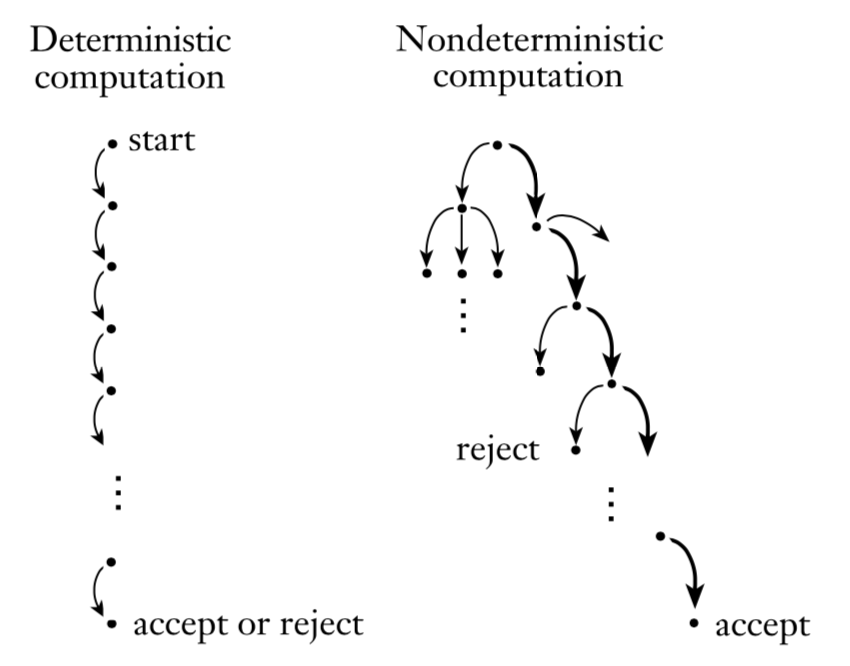
\includegraphics[width = 0.5\textwidth]{images/non-deterministic-turing-machine.png}
    \caption{Deterministic and non-deterministic Turing machine tree diagram.}
    \label{fig:non-deterministic-turing-machine}
\end{figure}

You can see a graphical representation of a non-deterministic Turing machine compared to a deterministic one. Informally, in a non-deterministic Turing machine there may exist several choices for the next state (and movement / writing of the head).

\begin{theorem}[]
    Every non-deterministic turing machine has an equivalent deterministic turing machine.
\end{theorem}

\begin{proof}
    The general idea for this proof is to consider the tree of all possible computations of a non-deterministic turing machine. We start from the root and do a breadth-first search and accept only if an accepting configuration is found. This can be done on a multitape turing machine, and hence there exists an equivalent deterministic turing machine.
\end{proof}

    \lecture{3}{10/10}

Here we introduce some termionlogy to make which will be more heavily utilised later in this course. When taking derivates of a multivariate function, say $f(x, y)$, we may right the variable(s) that we are holding as subscript in the bottom right. So if we differentiate $f$ with respect to $x$ (so we are holding $y$ constant) we write \[ \left(frac{\partial f}{\partial x}\right)_y. \] 

So we can now rewrite the chain rule for multivariate functions with this notation.

\[ \left((\frac{\partial f}{\partial x}\right)_y = \left(\frac{\partial u}{\partial x}\right)_y \left(\frac{\partial F}{\partial u}\right)_v + \left(\frac{\partial v}{\partial x}\right)_y\left(\frac{\partial F}{\partial v}\right)_u \] and \[ \left(\frac{\partial f}{\partial y}\right)_x = \left(\frac{\partial u}{\partial y}\right)_x \left(\frac{\partial F}{\partial u}\right)_v + \left(\frac{\partial v}{\partial y}\right)_x \left(\frac{\partial F}{\partial v}\right)_u. \]

\begin{example}
    Suppose $(r, \theta)$ are polar coordinates $(x, y)$ are cartesian coordinates, and \[ F(r, \theta) = r\cos\theta = x = f(x, y). \] Remember previously that
    \begin{align*}
        \frac{\partial r}{\partial x} &= \frac{x}{\sqrt{x^2 + y^2}} & \frac{\partial r}{\partial y} &= \frac{y}{\sqrt{x^2 + y^2}} \\
        \frac{\partial \theta}{\partial x} &= \frac{-y}{x^2 + y^2} & \frac{\partial \theta}{\partial y} &= \frac{x}{x^2 + y^2}. 
    \end{align*}
    And we have
    \begin{align*}
        \frac{\partial f}{\partial x} &= \frac{\partial}{\partial x} (x) = 1 \\
        \frac{\partial f}{\partial y} &= \frac{\partial}{\partial y} (x) = 0.
    \end{align*}
    We can use this result to confirm the chain rule.
    \begin{align*}
        \frac{\partial f}{\partial x} &= \frac{\partial r}{\partial x} \frac{\partial F}{\partial r} + \frac{\partial \theta}{\partial x} \frac{\partial F}{\partial \theta} \\
        &= \frac{x}{\sqrt{x^2 + y^2}} \frac{\partial}{\partial r} (r\cos{\theta}) - \frac{y}{x^2 + y^2} \frac{\partial}{\partial \theta} (r\cos{\theta}) \\
        &= \frac{x}{\sqrt{x^2 + y^2}} \cos{\theta} + \frac{y}{x^2 + y^2} r\sin{\theta} \\
        &= \frac{r\cos^2{\theta}}{r} + \frac{r^2 \sin^2{\theta}}{r^2} \\
        &= \cos^2{\theta} + \sin^2{\theta} = 1.
    \end{align*}
    This agrees with above. This can be done again for the other equation.
\end{example}

Sometimes we will write an application of the chain rule using just operators, so taking the polar coordinates example above we may write \[ \frac{\partial}{\partial x} = \frac{x}{\sqrt{x^2 + y^2}} \frac{\partial}{\partial r} - \frac{y}{x^2 + y^2} \frac{\partial}{\partial \theta}. \] This will be applied to two suitable functions $F$ and $f$.

\chapter{Vector calculus}

Lets start with some notation.

\begin{enumerate}
    \item $\R$, the set of all real numbers (think of this as a number line).
    \item $\R^n$, set of ordered $n$-tuples $(x_1, x_2, \ldots, x_n)$ where $x_i \in \R$ with $1 \leq i \leq n$. We can think of this as the coordinates of a point in $n$-dimesional cartesian space. The position vector of a point in $\R^n$ can be written in terms of the standard basis $\{ \bm{e_1}, \bm{e_2}, \ldots, \bm{e_n}\}$ as \[ \bm x = x_1 \bm{e_1} + x_2 \bm{e_2} + \ldots + x_n \bm{e_n} \] or more simply \[ \bm x = \sum_{i = 1}^n x_i \bm{e_i}. \]
\end{enumerate}

\begin{remark}[Einstein summation convention]
    According to this convention, if an index variable appear twice in a single term and is not otherwise defined, it implies summation over all values of the index. For example \[ y = \sum_{i = 1}^{3} c_ix^i = c_1x + c_2x^2 + c_3x^3 \iff y = c_ix^i. \]
\end{remark}

    \lecture{4}{20/1}

\begin{example}
    Integrate $f(x, y) = 4xy - y^3$ over $A$ where $A$ is the finite region
    between $y = x^3$ and $y = \sqrt x$ for $x \in [0, 1]$.
\end{example}

\begin{figure}[]
    \centering
    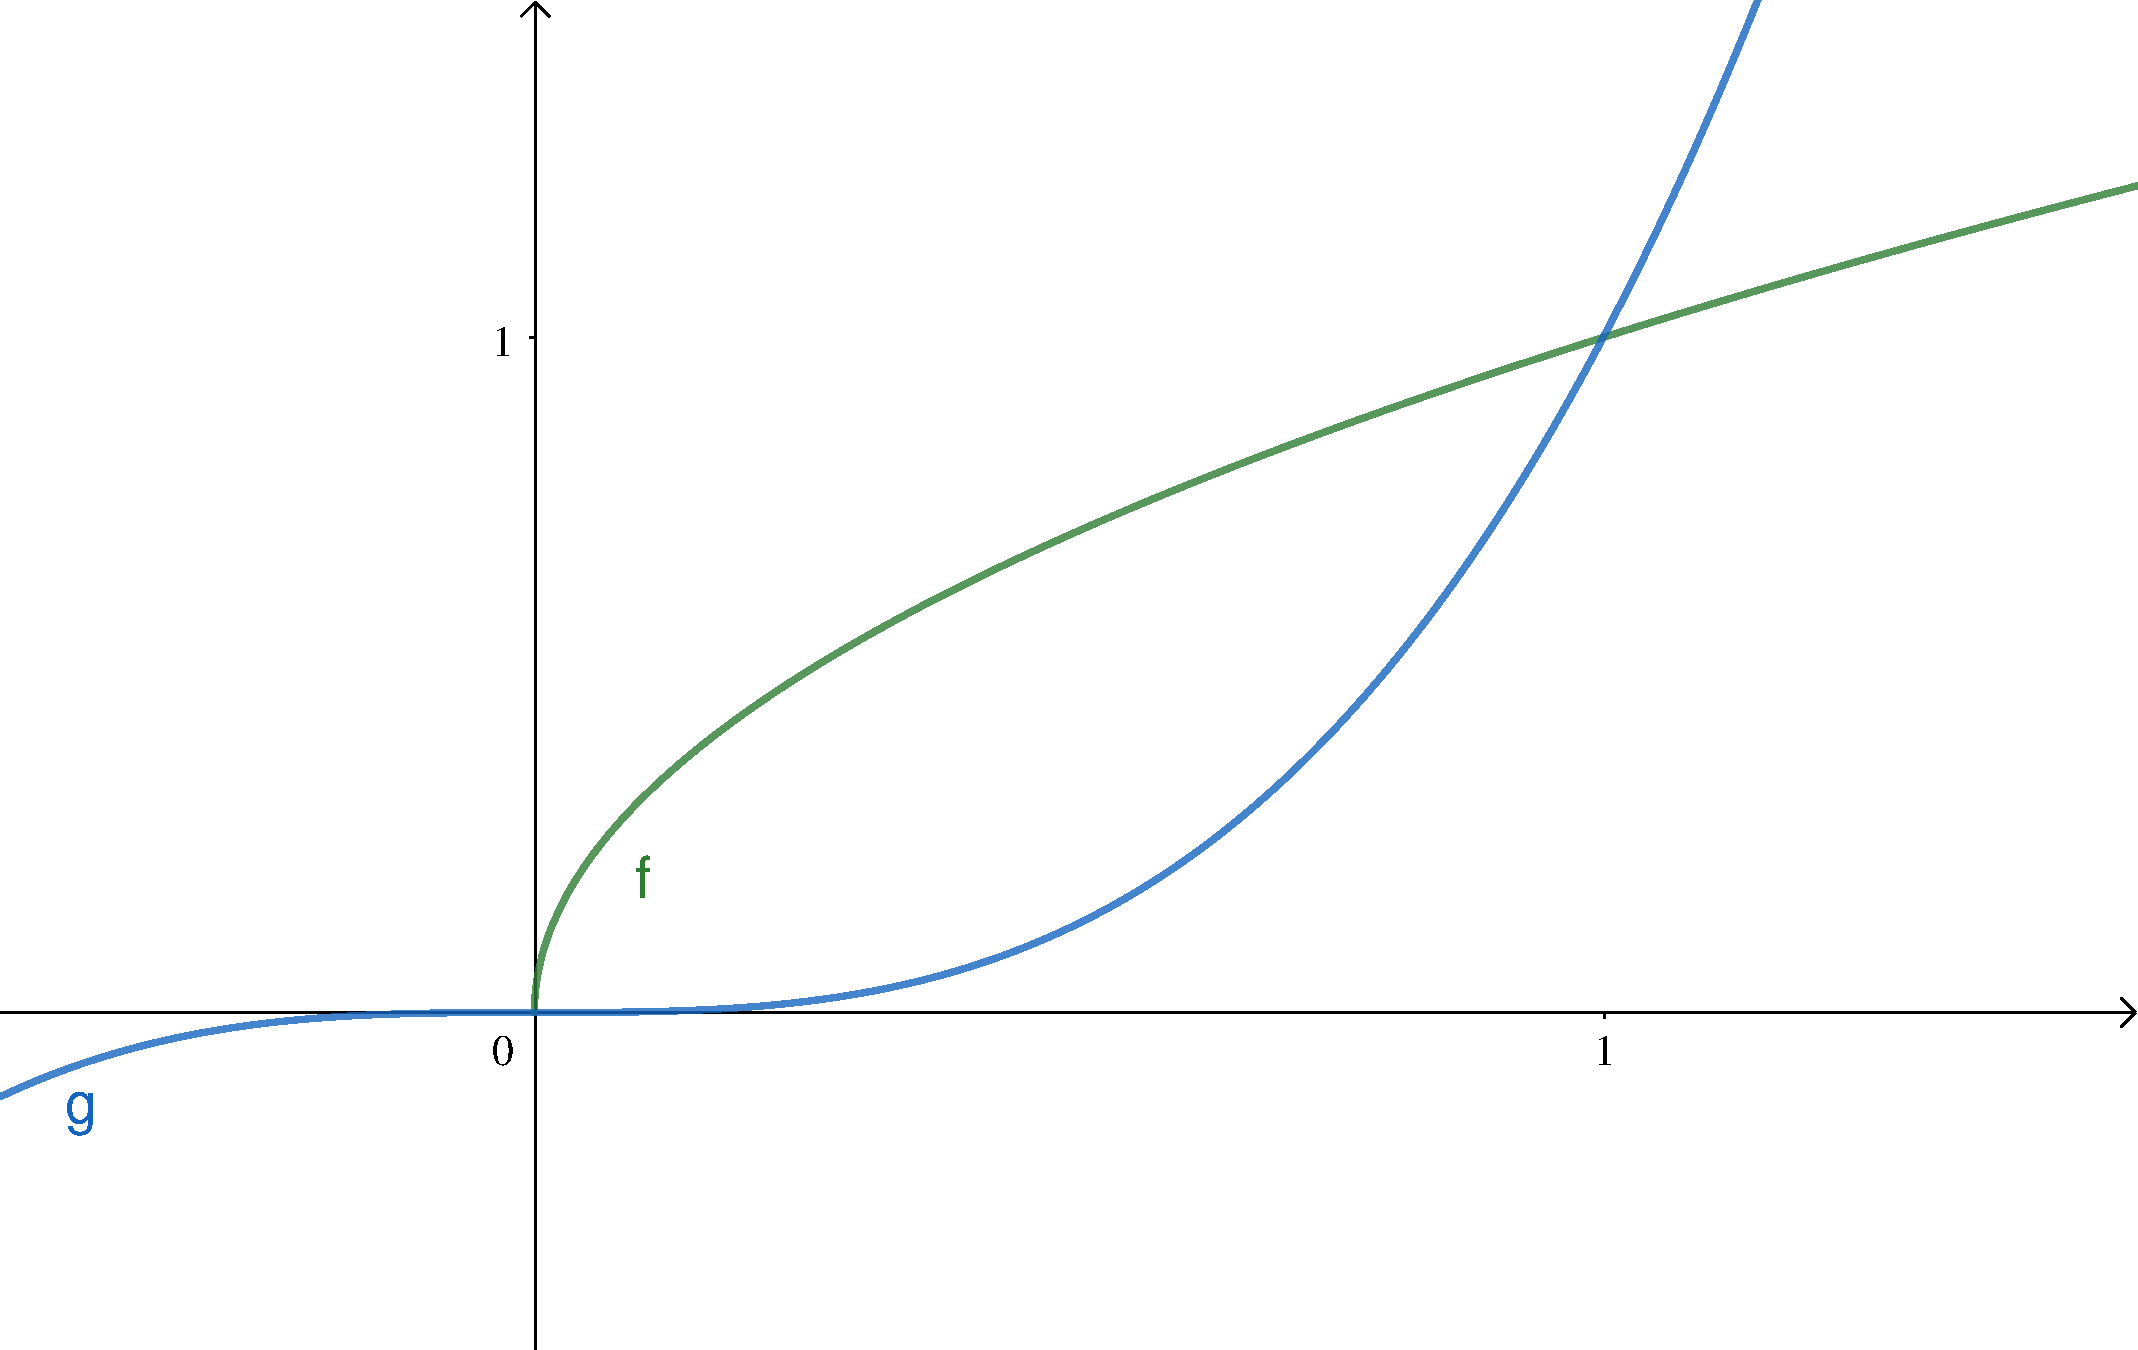
\includegraphics[width=0.8\linewidth]{images/fubini-ex-1.pdf}
    \caption{}
    \label{fig:fubini-ex-1}
\end{figure}

\begin{solution}
    The first thing we should do is draw $A$, as shown in Figure 
    \ref{fig:fubini-ex-1}.
    So we have
    \begin{align*}
        \int_A (4xy - y^3) \, dA
        &= \int_0^1 \int_{x^3}^{\sqrt x} (4xy - y^3) \, dy \, dx \\
        &= \int_0^1 \left(2xy^2 - \frac14y^4\right)^{\sqrt x}_{x^3} \, dx \\
        &= \int_0^1 (2x^2 - \frac14x^2 - 2x^7 + \frac14x^{12}) \, dx \\
        &= \left(\frac23x^3 -\frac1{12}x^3 - \frac14x^8 + 
            \frac1{52}x^{13}\right)_0^1 \\
        &= \frac23 - \frac1{12} - \frac14 + \frac1{52} = \frac{55}{156}.
    \end{align*}
    As the region $A$ is $x$-simple and $y$-simple,
    you can swap the order of integration and still get the same answer.
\end{solution}

\begin{example}
    Integrate $f(x, y) = e^{-x^2}$ over the triangle $A$ with
    vertices $(0,0)$, $(1,0)$, and $(1, 1)$.
\end{example}

\begin{solution}
    $A$ is clearly $x$-simple and $y$-simple, 
    so the order of integration does not matter.
    \begin{enumerate}
        \item 
            First attempt: we will attempt to integrate $x$ first.
            \[
                \int_A e^{-x^2} \, dA = \int_0^1 \int_y^1 e^{-x^2} \, dx \, dy;
            \]
            however, the antiderivative of $e^{-x^2}$ cannot be represented
            in terms of elementary functions.

        \item Second attempt: we will attempt to integrate $y$ first.
            \begin{align*}
                \int_A e^{-x^2} \, dA
                &= \int_0^1 \int_0^x e^{-x^2} \, dy \, dx \\
                &= \int_0^1 \left(ye^{-x^2}\right)^x_0 \, dx \\
                &= \int_0^1 \left(xe^{-x^2}\right) \, dx \\
                &= \left(-\frac12e^{-x^2}\right)^1_0 \\
                &= -\frac12e^{-1} + \frac12 \\
                &= \frac12\left(1-\frac1e\right).
            \end{align*}
    \end{enumerate}
\end{solution}

\begin{example}
    Integrate $f(x, y) = x^2 + y^2$ over $A = B_1(\bm 0)$.
\end{example}

\begin{solution}
    \begin{align*}
        \int_A(x^2 + y^2) \, dA
        &= \int_0^{2\pi} \int_0^1 r^2 \cdot r \, dr \, d\theta \\
        &= \int_0^{2\pi} \left(\frac14r^4\right)^{r = 1}_{r = 0} d\theta \\
        &= \int_0^{2\pi} \frac14 \, d\theta \\
        &= \left(\frac14\theta\right)^{2\pi}_0 = \frac{\pi}2
    \end{align*}
\end{solution}

\begin{example}
    Find the mass $M$ of air inside a hemispherical volume
    of radius $r$ centered at the origin, when the air density
    varys with height as $\rho = cz + \rho_0$ 
    ($c, \rho_0$ are constants).
\end{example}

\begin{solution}
    \begin{align*}
        M &= \int_0^r \int_{-r_z}^{r_z} 
        \int_{-\sqrt{r_z^2 - y^2}}^{\sqrt{r_z^2 - y^2}} \rho(z) \,dx\,dy\,dz \\
        \vdots \\
        M &= \int_0^r (cz + \rho_0) \pi (r^2 - z^2) \, dz \\
        \vdots \\
        M &= \pi \left( \frac c4 r^4 + \frac23 \rho_0 r^3 \right).
    \end{align*}
\end{solution}

\chapter{Line and surface integrals}
\section{Line integrals}

\begin{definition}[Regular arc]
    A \textbf{regular arc} is a parametrised curve $\bm x(t)$ for which
    the components $x_a(t)$ are continuous with continuous first derivatives,
    where $t$ lies in some (maybe infinite) interval $[\alpha, \beta]$.
\end{definition}

It is useful to consider \emph{regular curves} too, 
which is effectiveless just a series of regular arcs \emph{glued}
together.

\begin{definition}[Regular curve]
    A \textbf{regular curve} consists of a finite number of regular arcs
    joined end to end.
\end{definition}

    %! TEX root = master.tex

\section{Topological spaces}
\lecture{5}{18/10}

\begin{definition}[Topology]
	Let $X$ be a set.
	A \emph{topology} on $X$ is a subset $\tau \subset \mathcal P(X)$ which 
	satisfies the following:
	\begin{enumerate}
		\item $X, \varnothing \in \tau$;
		\item for $i \in I$, 
			$U_i \in \tau \implies \bigcup_{i \in I} U_i \in \tau$; and
		\item $U_1, U_2 \in \tau \implies U_1 \cap U_2 \in \tau$.
	\end{enumerate}
	The elements of $\tau$ are called the \emph{open subsets} of $X$.
	If $A \subset X$ and $X \setminus A \in \tau$, we say that $A$ is 
	\emph{closed}.
\end{definition}

\begin{examples}
	\hfill
	\begin{enumerate}
		\item 
		Let $(M,d)$ be a metric space.
		Then the collection of open sets as defined in the last section defines 
		a topology.
		This is confirmed by the previous lemma.

		\item
		$(X, \mathcal P)$ defines a topological space, namely the 
		\emph{discrete} topology on $X$.

		\item
		$(X, \left\{ \varnothing, X \right\})$ 
		also defines a (boring) topological
		space, namely the \emph{indiscrete} or \textbf{trivial} topology 
		on $X$.

		\item
		Let $X = \Z_{\geq 0}$ and
		\[
			\tau = \left\{ \varnothing \right\} \cup
			\left\{ 
				U \subset X: \left\lvert X \setminus U \right\rvert < \infty 
			\right\}.
		\]
		We can see that $\varnothing, X \in \tau$.
		Simiarly, if $U_1, U_2 \in \tau$, then clearly $U_1 \cap U_2 \in \tau$
		as 
		$X \setminus (U_1 \cap U_2) = (X \setminus U_1) \cup (X \setminus U_2)$.
		Now let $U_i \in \tau$ with $i \in I$, $I$ being some arbitrary 
		labelling set.
		If all $U_i = \varnothing$, then $U_{i \in I} U_i \in \tau$.
		Now assume that there is $j \in I$ such that $U_j \neq \varnothing$.
		Then
		\[
			X \setminus \bigcup_i U_i 
			= \bigcap_i (X \setminus U_i) 
			\subset X \setminus U_j
		\]
		and hence is finite.
		Therefore, $\tau$ is a topology on $X$.

		\item 
		Let $(X, \tau)$ be a topological space and $A \subset X$.
		Then 
		\[ 
			\tau_A = \left\{ A \cap U: U \in \tau \right\}
		\]
		is a topology  on $A$ called the \emph{induced} topology or 
		\emph{subspace} topology.
	\end{enumerate}
\end{examples}

\begin{problem}
	Show that the metrics $d_p$ and $d_\infty$ for $p \in [1,\infty)$ both 
	induce the same topology on $\R^n$.
\end{problem}

\begin{solution}
	Recall
	\begin{align*}
		d_p(x,y)
			&= \sum_{i=1}^n \left( 
				\left\lvert x_i - y_i \right\rvert^p 
			\right)^{\frac1p} \\
		d_\infty(x,y)
			&= \max\left\{ 
				\left\lvert x_i - y_i \right\rvert: 
				i \in \left\{ 1, \ldots, n \right\}
			\right\}.
	\end{align*}
	Clearly we have $d_\infty(x,y) < d_p(x,y)$.
	Simiarly, $d_p(x,y) < \sfrac1{n^{\frac1p}} d_\infty(x,y)$ and so if a 
	subset is open with $d_p(x,y)$, it is also open with $d_\infty(x,y)$ and
	vice versa.
	Therefore, both metrics (regardless of choice of $p$ induce the same
	topology. 
\end{solution}

    \section{Cauchy's integral formula}
\lecture{6}{29/1}

\begin{proposition}
    If $\gamma: [a,b] \to \C$ is a contour and 
    $\{f_n\}_{n = 1}^\infty$
    is a sequence of continuous functions 
    $f_n: \gamma([a,b]) \to \C$
    converging uniformly on $\gamma([a,b])$
    to a continuous function 
    $f: \gamma([a,b]) \to \C$
    then
    \[
        \lim_{n \to \infty} \int_\gamma f_n(z) \,dz
        = \int_\gamma f(z) \,dz.
    \]
\end{proposition}

\begin{proof}
    The proof to this comes from the analogous fact
    from Analysis I.
\end{proof}

\begin{theorem}[Cauchy's integral formula]
    Let $r > 0$, $a \in \C$, $f: B_r(a) \to \C$ be holomorphic.
    Let $\rho \in (0, r)$, then for all $w$ such that
    $\lvert w - a \rvert < \rho$ (that is, $w \in B_\rho(a)$) then
    \[ 
        f(w) = \frac1{2\pi i} 
        \int_{\lvert z - a \rvert = \rho} \frac{f(z)}{z - w} \,dz.
    \]
\end{theorem}

This is quite peculiar; it tells us that holomorphic functions are
\emph{defined} by a boundary.

\begin{proof}
    We define
    \[
        g(z) =
        \begin{cases}
            \frac{f(z) - f(w)}{z - w} & z \neq w \\
            f'(w) & z = w.
        \end{cases}
    \]
    $g$ is holomorphic away from $w$ and
    \[
        \lim_{z \to w} \frac{f(z) - f(w)}{z - w} = f'(w)
    \]
    and so $g$ is continuous at $w$ and thus $g$ is continuous.
    Note that $B_r(a)$ is starlike.
    Hence, we have met the requirements fore Cauchy's theorem for
    starlike domains and thus
    \begin{align*}
        \int_{\lvert z - a \rvert = \rho} g(z) \,dz &= 0 \\
        \int_{\lvert z - a \rvert = \rho}
            \frac{f(z) - f(w)}{z - w} \,dz &= 0 \\
        \int_{\lvert z - a \rvert = \rho} \frac{f(z)}{z - w} \,dz
        &= \int_{\lvert z - a \rvert = \rho} \frac{f(w)}{z - w} \,dz.
    \end{align*}
    For $\lvert z - a \rvert = \rho$
    \begin{align*}
        \frac1{z - w} 
        &= \frac1{(z-a)\left(1 - \frac{w-a}{z-a}\right)} \\
        &= \frac1{z-a} \sum_{n=0}^\infty 
        \left(
            \frac{w-a}{z-a}
        \right)^n \\
        &= \sum_{n = 0}^\infty \frac{(w - a)^n}{(z - a)^{n + 1}}
    \end{align*}
    which is valid as 
    $\left\lvert \frac{w-a}{z-a} \right\rvert 
    = \frac{\lvert w - a \rvert}{\rho} < \frac{\rho}{\rho} = 1$.
    So
    \begin{align*}
        \int_{\lvert z - a \rvert = \rho} \frac{f(z)}{z - w} \,dz
        &= \int_{\lvert z - a \rvert = \rho} \frac{f(w)}{z - w} \,dz \\
        &= \int_{\lvert z - a \rvert = \rho} f(w) 
        \left(
            \sum_{n = 0}^\infty \frac{(w - a)^n}{(z - a)^{n + 1}}
        \right)
        \,dz.
    \end{align*}
    $\sum_{n = 0}^\infty \frac{(w - a)^n}{(z - a)^{n + 1}}$ converges
    uniformly on $\lvert z - a \rvert = \rho$ by the $M$-test.
    Hence, by the previous proposition
    \begin{align*}
        \int_{\lvert z - a \rvert = \rho} \frac{f(z)}{z - w} \,dz
        &= f(w) \sum_{n = 0}^\infty 
            \int_{\lvert z - a \rvert = \rho} 
            \frac{(w - a)^n}{(z - a)^{n + 1}}
            \,dz \\
        &= f(w) \sum_{n = 0}^\infty (w - a)^n 
            \int_{\lvert z - a \rvert = \rho}
            \frac1{(z-a)^{n+1}} \,dz.
    \end{align*}
    We have seen before that
    \[
        \int_{\lvert z \rvert = 1} \frac{1}{z^{n+1}} \,dz =
        \begin{cases}
            2\pi i & n = 0 \\
            0 & n \neq 0.
        \end{cases}
    \]
    The same result holds for any other ball.
    Hence
    \[
        \int_{\lvert z - a \rvert = \rho} \frac{f(z)}{z - w} \,dz = f(w) \cdot 2\pi i.
    \]
\end{proof}

\chapter{Features of holomorphic functions}
\section{The Cauchy-Taylor theorem and integral formula for derivatives}

Recall that power series can be differentiated in their radius of convergence;
that is, they give holomorphic functions there.
In fact, all holomorphic functions are given locally by a power series.

\begin{theorem}[Cauchy-Taylor theorem]
    Let $r > 0$, $a \in \C$, and $f: B_r(a) \to \C$ be holomorphic.
    Then $f$ has a convergent power series expansion; that is,
    \[
        f(z) = \sum^{\infty}_{n = 0} c_n (z - a)^n \tag{$\dagger$}
    \]
    for all $z \in B_r(z)$ where
    \[
        c_n = \frac{1}{2\pi i}    
        \int_{\lvert z - a \rvert = \rho}
        \frac{f(z)}{(z - a)^{n + 1}} \,dz
    \]
    for any $\rho \in (0,r)$.
\end{theorem}

We call $(\dagger)$ the taylor series of $f$ at $a$.

\begin{proof}
    For any $0 < \rho < r$ we have
    \[
        f(w) = \frac{1}{2\pi i} \int_{\lvert z - a \rvert = \rho}
        \frac{f(z)}{z - w} \,dz
    \]
    for all $w \in B_{\rho}(a)$
    by Cauchy's integral formula.
    By the geometric series formula we get
    \[
        f(w) = \frac{1}{2\pi i} \int_{\lvert z - a \rvert = \rho}
        f(w) \sum^{\infty}_{n = 0} \frac{(w - a)^n}{(z - a)^{n + 1}} \,dz 
    \]
    so the previous proof (for uniform convergence) and the previous
    proposition tells us
    \[
        f(w) = \frac{1}{2\pi i} \sum^{\infty}_{n = 0} (w - a)^n
        \int_{\lvert z - a \rvert = \rho} \frac{f(z)}{(z - a)^{n + 1}} \,dz
        = \sum^{\infty}_{n = 0} c_n (w-a)^n.
    \]
    Therefore, $f$ has a power series expansion of $B_{\rho}(a)$ so
    \[
        c_n = f^{(n)}(a) \cdot \frac1{n!}
    \]
    which does not depend on $\rho$.
    Now, as for all $w \in B_r(a): w \in B_{\rho}(a)$ for some $\rho < r$
    and hence holds for $B_r(a)$.
\end{proof}

    \lecture{7}{24/2}

    %! TEX root = master.tex
\lecture{8}{5/11}

\begin{definition}[Ring of integers]
	For a number field $K$, we define
	\[
		\mathcal O_K = K \cap \overline\Z,
	\]
	the \emph{ring of integers of $K$}.
\end{definition}

$\mathcal O_K$ is indeed a ring as it is the intersection of a field
and a ring.

\begin{lemma}[]
	$\mathcal O_\Q = \Z$.
\end{lemma}

\begin{proof}
	As $\Z$ is contained within $\overline\Z$ and $\Q$, we have
	$\Z \subset \mathcal O_\Q$.
	Now let $\alpha \in \mathcal O_\Q$.
	Since $\alpha \in \Q$, there is minimal polynomaial $p(x) \in \Q[x]$ 
	with $\deg p = 1$;
	that is, $p(x) = x - \alpha$.
	As $\alpha \in \overline\Z$, we have that $p(x) \in \Z[x]$, and so
	$\alpha \in \Z$.
\end{proof}

\begin{lemma}[]
	Let $K$ be a number field. Then
	\[
		K =
		\left\{ 
			\frac{\alpha}m : 
			\alpha \in \mathcal O_K, m \in \Z \setminus \left\{ 0 \right\} 
		\right\}.
	\]
\end{lemma}

\begin{proof}
	Let $\beta \in K$.
	As $\beta$ is algebraic, there is $a_0, \ldots, a_n \in \Z$
	such that
	\[
		a_n\beta^n + \ldots + a_0 = 0,
	\]
	with $a_n \neq 0$.
	We multiply this by $a_n^{n-1}$ to get
	\[
		(a_n\beta)^n
		+ a_{n-1}(a_n\beta)^{n-1}
		+ \ldots
		+ a_1 a_n^{n-1} (\alpha_n\beta) + a_n^{n-1}a_0
		= 0
	\]
	and so $\alpha = a_n\beta$ is an algebraic integer.
	Paired with the fact that $\alpha \in K$, we see
	that $\alpha \in \mathcal O_K$.
	That is, $\beta = \frac{\alpha}{a_n}$, which shows
	our statement by taking $m = a_n$.
\end{proof}

\subsection{Quadratic fields}

\begin{definition}[Square-free integer]
	A \textbf{square-free integer} is an integer which is divisible by
	no perfect square other than 1.
\end{definition}

\begin{proposition}[]
	Let $K$ be an extension field of $\Q$ of degree 2.
	Then there is some square-free integer $d$ such that $K = \Q(\sqrt d)$.
\end{proposition}

\begin{definition}[Quadratic field]
	A \textbf{quadratic field} is a field $K = \Q(\sqrt d)$.
	If $d > 0$, $K$ is a \emph{real quadratic field}.
	If $d < 0$, $K$ is a \emph{imaginary quadratic field}.
\end{definition}

We will work towards determining the ring of integers for quadratic fields.

\begin{lemma}[]
	Let $K = \Q(\sqrt d)$ with $1 \neq d \equiv 1 \pmod 4$.
	Then
	\begin{enumerate}
		\item
			\[
				\Z \left[ \frac{1+\sqrt d}2 \right] 
				\subset \mathcal O_K;\;\text{and}
			\]

		\item
			\[
				\Z \left[
					\frac{1 + \sqrt d}2
				\right] = \left\{
					\frac{r + s\sqrt d}2:
					r,s \in \Z, r \equiv s \pmod 2
				\right\}.
			\]
	\end{enumerate}
\end{lemma}

\begin{proof}
	$(i)$: it is enough to show that $\frac{1 + \sqrt d}2 \in \mathcal O_K$
	since $\mathcal O_K$ is a ring.
	Clearly $\frac{1 + \sqrt d}2 \in K$ and it is a root of
	$x^2 - x - \frac{d-1}4 \in \Z[x]$.
	$(ii)$: let $\theta = \frac{1 + \sqrt d}2$.
	Observe that $\Z[\theta] = \Z + \theta\Z$ as
	$\theta^2 = \theta + \frac{d-1}4$.
	So if $\beta \in \Z[\theta]$ then there is $x,y \in \Z$ such that
	$\beta = x + y\theta$ or equivalently
	$
		\frac{(2x+y)+y\sqrt d}{2}.
	$
	Since $2x + y \equiv y \pmod 2$, we can take $r = 2x + y$ and
	$s = y$ to conclude the first inclusion.
	Conversely, if $\beta = \frac{r+s\sqrt d}2$ with $r,s \in \Z$ and
	$r \equiv s \pmod 2$ then 
	\[
		\beta = \frac{r-s}2 + s\left( 
			\frac{1 + \sqrt d}{2}  
		\right) \in \Z + \Z\theta = \Z[\theta].\qedhere
	\]
\end{proof}

We are ready to look at the ring of integers of quadratic fields.

\begin{theorem}[]
	Let $d$ be a square-free integer and $K = \Q(\sqrt d)$.
	Then
	\[
		\mathcal O_K =
		\begin{cases}
			\Z[\sqrt d] & d \equiv 2,3 \pmod 4, \\
			\Z\left[\frac{1 + \sqrt d}2\right] & d \equiv 1 \pmod 1. \\
		\end{cases}
	\]
\end{theorem}

\begin{proof}
	If $d \equiv 1 \pmod 4$, then 
	$\Z\left[\frac{1+\sqrt d}2\right] \subset \mathcal O_K$.
	If $d \equiv 2,3 \pmod 4$, then $\Z[\sqrt d] \subset \mathcal O_K$ as
	$\sqrt d \in \mathcal O_K$.

	Now we show the other inclusion.
	We let $\alpha = \frac{a + b\sqrt d}c \in \mathcal O_K$ with 
	$a,b,c \in \Z$.
	If $b = 0$, then $\alpha \in \Q \cap \overline\Z = \Z$.
	Now assume $b \neq 0$.
	Without loss of generality, we assume $\gcd(a,b,c) = 1$ and
	$c \in \N$.
	Then the minimum polynomial of $\alpha$ is given by
	\[
		p(x) = \left( 
			x - \frac{a + b\sqrt d}c 
		\right) \left( 
			x - \frac{a - b\sqrt d}c 
		\right)
		= x^2 - \frac{2a}c x + \frac{a^2 - b^2d}{c^2}
		\in \Z[x].
	\]
	Thus $\frac{2a}c, \frac{a^2 - b^2d}{c^2} \in \Z$.
	Now let $p$ be prime such that $p \mid a,c$.
	Then $p^2 \mid b^2d$.
	As $d$ is square free, $p \mid b^2$ and then
	$p \mid a,b,c$. 
	That is, $\gcd(a,b,c) > 1$; a contradiction.
	Hence $\gcd(a,c) = 1$.
	Thus $c \in \left\{
		1,2
	\right\}$.
	If $c=1$, then $\alpha = a+b\sqrt d \in \Z[\sqrt d]$ and
	$\alpha \in \Z\left[\frac{1 + \sqrt d}2\right]$ 
	since $a + b\sqrt d = (a - b) + 2b \frac{1 + \sqrt d}2$.
	If $c=2$, then $a$ and $b$ are odd.
	Furthermore, as $\frac{a^2 - b^2d}4 \in \Z$,
	$a^2 - b^2d \equiv 0 \pmod 4$.
	As $a$ and $b$ are odd, $a^2 \equiv b^2 \equiv 1 \pmod 4$.
	Hence $d \equiv 1 \pmod 4$.
\end{proof}


    % this is where I started going back to lectures after being ill
\lecture{9}{5/11}

\begin{theorem}[Eisenstein's criterion]
    Let $f(x) = a_0 + a_1 x + \ldots + a_n x^n \in \Z$ with a prime $p$ such that
    \[ p \nmid a_n, \quad p \mid a_0, \ldots, a_{n - 1}, \quad p^2 \nmid a_0 \]
    then $f(x)$ is irreducible in $\Q[x]$.
\end{theorem}

\begin{example}
    Let $p \in \Z$ be a prime number. The polynomial
    \[ \Phi_p(x) = x^{p-1} + x^{p-2} + \ldots + x + 1 = \frac{x^p}{x - 1} \]
    is called the $p$th cyclotomic polynomial and it is irreducible (and we will prove it).
    Set 
    \begin{align*}
        f(x) &= \Phi_p(x + 1) \\
             &= \frac{(x + 1)^{p - 1}}{(x + 1) - 1} \\
             &= \frac{x^p + \binom{p}{1}x^{p - 1} + \ldots + \binom{p}{1}x + 1 - 1}{x} \\
             &= x^{p - 1} + px^{p - 2} + \ldots + \binom{p}{2}x + p.
    \end{align*}
    Observe that $1 \leq k \leq p - 1 \implies p \mid \binom pk$. So
    \[ p \mid a_0, a_1, \ldots, a_{p - 2}, \]
    $a_{p - 1} = 1$, $a_0 = p$, and $p^2 \nmid a_0$.
    So by Eisenstein's criterion we have that $f(x)$ is irreducible in $\Q[x]$.
\end{example}

\section{Prime elements}

\begin{definition}[Prime element]
    Let $F$ be a commutative ring. Then $a \in R$ is called a \textbf{prime element} if
    \begin{enumerate}
        \item $a \neq 0$ and $a$ is not a unit; and
        \item $a \mid xy \implies a \mid x \;\text{or}\; a \mid y$.
    \end{enumerate}
\end{definition}

\begin{proposition}[]
    Let $R$ be an integral domain. If $a \in R$ is prime then it is irreducible.
\end{proposition}

\begin{proof}
    So we have $a \in R$ prime. 
    So $a \neq 0$, $a$ is not a unit, and $a \mid bc \implies a \mid b \;\text{or}\; a \mid c$.
    We have
    \[ a = bc \implies a \mid bc \implies a \mid b \;\text{or}\; a \mid c \]
    and $a \mid b \implies b = ax$ for some $b \in R$. So
    \[ a = axc \implies a(1 - xc) = 0 \implies xc = 1; \]
    hence, $x$ and $c$ are units. This can be similarly shown that $a \mid c \implies b \;\text{is a unit}$.
\end{proof}

\begin{example}
    Let $F$ be a field. Then $f(x) \in F[x]$ is irreducible if and only if $f$ is prime.
\end{example}

\begin{proof}
    \begin{description}
        \item[$\impliedby$] Above.
        \item[$\implies$] We have $f(x) \in F[x]$ where $F$ is a field and $f$ is irreducible. 
            Hence $f(x) \neq 0$ and not a unit. 
            Suppose $f \mid hg$. 
            Suppose $f \nmid g$. Then
            \[ \gcd{(f, g)} \mid f \implies \gcd{(f, g)} = 1. \]
            By the Euclidean algorithm there exists $f_1$ and $g_1$ such that
            \begin{align*}
                f(x) f_1(x) + g(x) g_1(x)           &= 1    \\
                f(x) f_1(x) h(x) + g(x) g_1(x) h(x) &= h(x);
            \end{align*}
            hence $f(x) \mid \text{LHS}$ and so $f(x) \mid \text{RHS}$.
    \end{description}
    %todo this proof is a little sketchy.
\end{proof}

\begin{example}[Irreducibility $\not\implies$ prime]
    Consider $R = \Z[\sqrt{-5}] \subset \C$. We claim that $2$ is irreducible but not prime. Consider $N: \R \to \Z$ defined by
    \[ N(a + b\sqrt{-5}) = (a + b\sqrt{-5})(a - b\sqrt{-5}) = a^2 + 5b^2. \]
    Let $x_1 = a + b\sqrt{-5}$ and $x_2 = c + d\sqrt{-5}$.
    Then
    \[ N(x_1, x_2) = x_1 x_2 \overline{x_1x_2} = x_1 \bar x_1 x_2 \bar x_2 = N(x_1)N(x_2) \]
    and hence $N$ is multiplicative. Suppose $2 = ab$ where $a, b \in \Z[\sqrt{-5}]$.
    Then 
    \[ 4 = N(2) = N(ab) = N(a)N(b). \]
    Let $a = x + y\sqrt{-5}$ and $b = z + w\sqrt{-5}$. Then 
    \[ 4 = (x^2 + 5y^2)(z^2 + 5w^2). \]
    So
    \[
        x^2 + 5y^2 =
        \begin{cases}
            1 & x= pm 1, y = 0 \\
            2 & \text{no solutions} \\
            4 & x = \pm 2, y = 0;
        \end{cases}
    \]
    hence as when $x = \pm 2, y = 0$, it is irreducible. But $2$ is clearly not prime as
    \[ 2 \mid (1 - \sqrt{-5}(1 + \sqrt{-5}) = 6 \]
    implies that $2x = 1$, which is not possible for $x \in \Z$. So $2$ is irreducible but not prime in $R$.
    %todo again rocky proof but I believed it in lectures
\end{example}

    %! TEX root = master.tex
\lecture{10}{12/11}

\begin{theorem}[]
	For a cyclotomic field $K$ we have
	$[K:\Q] = \phi(n)$ and $\mathcal O_K = \Z[\zeta]$.
\end{theorem}

Here $\phi$ denotes Euler's totient function.
It denotes the order of the group $\left( 
	\Z/n\Z 
\right)^\times$ and is determined by the following rules:
\begin{enumerate}
	\item $\phi(nm) = \phi(n) \phi(m)$;
	\item $\phi(p^r) = (p-1)p^{r-1}$; and
	\item $\phi(1) = 1$.
\end{enumerate}

\section{Euclidean domains, principal ideal domains, and unique factorisation
domains}

\begin{definition}[Integral domain]
	An \emph{integral domain} is a commutative ring $R$ such that for every
	$a, b \in R$,
	\[
		ab = 0 \implies a = 0 \;\text{or}\; b = 0.
	\]
\end{definition}

Observe that for any number field $K$,
$\mathcal O_K \subset K$ and is an integral domain.

\begin{definition}[Euclidean function]
	Let $R$ be an integral domain.
	A \emph{Euclidean function} (or \emph{norm}) for $R$ is a function
	$\varphi: R \setminus \left\{
		0
	\right\} \to \N \cup \left\{
		0
	\right\}$ such that
	\begin{enumerate}
		\item for every $a, b \in R \setminus \left\{
			0
		\right\}$ such that $b \mid a \implies \varphi(b) \leq \varphi(a)$; and
		
		\item for every $a \in R$ and $b \in R \setminus \left\{
			0
		\right\}$ there is $q, r \in R$ such that
		$a = bq + r$ with $r = 0$ or $\varphi(r) < \varphi(b)$.
	\end{enumerate}
\end{definition}

\begin{definition}[Euclidean domain]
	An integral domain for which a Euclidean function exists is called a
	\emph{Euclidean domain} (ED).
\end{definition}

\begin{examples}
	\begin{enumerate}
		\item $\Z$ is a Euclidean domain.
			Indeed, the map defined by $a \mapsto \left\lvert a \right\rvert$
			is a Euclidean functioun.

		\item $\Q[x]$ is also a Euclidean domain.
			Indeed, the map $f(x) \mapsto \deg{f(x)}$.
	\end{enumerate}
\end{examples}

\begin{lemma}[]
	Consider the Gaussian integers, $K = \Q(i)$.
	The ring of Gaussian integers $\mathcal O_K = \Z[i]$ is a
	Euclidean domain with Euclidean function
	\[
		\varphi(x) = \operatorname{N}_{K/\Q}(x).
	\]
\end{lemma}

\begin{proof}
	For a quadratic field $K = \Q(\sqrt d)$,
	we have seen that $\operatorname{N}_{K/\Q}(a + b\sqrt d) = a^2 - db^2$
	for $a,b \in \Q$.
	Here we take $d = -1$.
	We have to check that $\varphi$ is actually a Euclidean function.
	Let $r,s \in \Z[i] \setminus \left\{
		0
	\right\}$.
	Then as $r \mid s$, $s = ra$ for some $a \in \Z[i]$.
	Then
	\begin{align*}
		N(s)
		&= N(ra) \\
		&= N(r) N(a) \\
		&\geq N(r).
	\end{align*}
	So $(i)$ holds.
	Now for $(ii)$: consider $x, y \in \Z[i]$ with $y \neq 0$.
	Then $\frac xy = a' + b'i$, $a', b' \in \Q$.
	Let $a, b \in \Q$ such that
	\[
		\left\lvert a - a' \right\rvert \leq \frac12, \qquad
		\left\lvert b - b' \right\rvert < \frac12.
	\]
	Set $q = a + bi$.
	Then
	\[
		x = qy + ((a' - a) + (b' - b)i)y = x - qy.
	\]
	Furthermore
	\begin{align*}
		\operatorname{N}_{K/\Q}(((a'-a) + (b'-b)i)y)
		&= \operatorname{N}_{K/\Q}((a' - a) + (b' - b)i)
			\operatorname{N}_{K/\Q}(y) \\
		&= ((a'-a)^2 + (b'-b)^2)
			\operatorname{N}_{K/\Q}(y) \\
		&\leq \frac12 \operatorname{N}_{K/\Q}(y) \\
		&< \operatorname{N}_{K/\Q}(y)
	\end{align*}
	as $y \neq 0$ if and only if $N_{K/\Q}(y) \neq 0$.
\end{proof}

    \lecture{11}{4/2}

We need to check whether $\phi(\bm x)$ satisfies $\bm F = \nabla \phi$.
\begin{align*}
    \frac{\partial\phi}{\partial x}
    &= \lim_{\delta x \to 0} 
        \frac{\phi(\bm x + \bm e_1 \delta x) - \phi(\bm x)}{\delta x} \\
    &= \lim_{\delta x \to 0} 
        \left(
            \frac{1}{\delta x} 
            \left(
                \int_{\bm x_0}^{\bm x + \bm e_1 \delta x}
                \bm F \cdot d\bm x
                + \int_{\bm x_0}^{\bm x} 
                \bm F \cdot d\bm x
            \right)
        \right).
\end{align*}
We see that
\[
    \int_{\bm x_0}^{\bm x + \bm e_1 \delta x} \bm F \cdot d\bm x
    = \int_{\bm x_0}^{\bm x} \bm F \cdot d\bm x 
    = \int_{\bm x}^{\bm x + \bm e_1 \delta x} \bm F \cdot d\bm x
\]
hence
\[
    \frac{\partial \phi}{\partial x}
    = \lim_{\delta x \to 0}
    \left(
        \frac{1}{\partial x} 
        \int_{\bm x}^{\bm x + \bm e_1 \delta x}
        \bm F \cdot d\bm x
    \right).
\]
We can parametrise this as 
\[
    \bm x(t) = (x + t, y, z), \qquad t \in [0,\delta x]
\]
where
$\frac{d\bm x}{dt} = \bm e_1$.
So
\begin{align*}
    \frac{1}{\delta x}
        \int_{\bm x}^{\bm x + \bm e_1 \delta x} \bm F \cdot d\bm x
    &= \frac{1}{\delta x} \int_0^{\delta x} 
        \bm F(x + t, y, z) \cdot \frac{d\bm x}{dt} \,dt \\
    &= \frac{1}{\delta x} \int_0^{\delta x} 
        F_1(x + t, y, z) \,dt \\
    &= \frac{1}{\delta x} \int_0^{\delta x} 
        \left(
            F_1 \delta x 
            + \frac12 \delta x^2 \frac{\partial F_1}{\partial x} 
            + \ldots
        \right)
        \,dt \\
    &= \frac{1}{\delta x} \int_0^{\delta x}
        F_1(x,y,z) + \frac{\delta x}{2} \frac{\partial F_1}{\partial x} + \ldots \\
    &\to \frac{1}{\delta x} \int_0^{\delta x} F_1(x,y,z)
\end{align*}
as $\delta x \to 0$ so 
\[
    \frac{\partial\phi}{\partial x} = F_1
\]
and similarly
\[
    \frac{\partial\phi}{\partial y} = F_2, \qquad
    \frac{\partial\phi}{\partial z} = F_3.
\]

$\phi$ (or $-\phi$) is called the \textbf{scalar potential}.

\begin{definition}[Closed]
    Let $\bm F$ be a vector field.
    $F$ is \textbf{closed} if $\nabla \times \bm F = \bm 0$.
\end{definition}

\begin{definition}[Exact]
    Let $\bm F$ be a vector field.
    $F$ is \textbf{exact} if there exists some scalar field $\phi$
    such that $F = \nabla\phi$.
\end{definition}

\begin{remark}
    Let $\bm F$ be a vector field.
    Then
    \[
        F \;\text{is exact}\; \implies F \;\text{is closed}.
    \]
    If we are in a simply connected domain, then
    \[
        \implies F \;\text{is closed}\; \implies F \;\text{is exact}.
    \]
    If our region has suitable \emph{holes}, this may fail.
\end{remark}

Finally, lets note that if $\bm F = \nabla\phi$
then path independence follows directly.

\begin{theorem}[]
    If $\bm F = \nabla\phi$ for some scalar field $\phi$
    and $C$ is a curve from $\bm x = \bm a$ to $\bm x = \bm b$
    then
    \[
        \int_C \bm F \cdot d\bm x = \phi(b) - \phi(a).
    \]
\end{theorem}

\begin{proof}
    Follows from the chain rule.
\end{proof}

\begin{example}
    Compute
    \[
        I = \int_C \bm F \cdot d\bm x
    \]
    where
    \[
        \bm F =
        \begin{pmatrix}
            y\cos(xy)             \\
            x\cos(xy) - z\sin(yz) \\
            -y\sin(yz)            \\
        \end{pmatrix}
    \]
    and $C$ is specified by $t \mapsto \bm x(t)$ where
    \[
        \bm x(t) =
        \begin{pmatrix}
            \frac{\sin t}{\sin t} \\
            \frac{\log(t + t)}{\log 2} \\
            \frac{1 - e^t}{1 - e} \\ 
        \end{pmatrix}
    \]
    with $t \in [0,1]$.
\end{example}

\begin{solution}
    Note that $\bm x(0) = (0,0,0)$ and $\bm x(1) = (1,1,1)$.
    We compute $\nabla \times \bm F = 0$ in all of $\R^3$ (trust me).
    So $\bm F = \nabla \phi$ for some $\phi$.
    So we have $\phi_x = F_1$, $\phi_y = F_2$, and $\phi_z = F_3$.
    Consider $\phi_x$, we have
    \[
        \frac{\partial\phi}{\partial x} = y\cos(xy)
        \implies \phi(x,y,z) = \sin(xy) + f(y,z).
    \]
    Then
    \begin{align*}
        \frac{\partial}{\partial y} (\sin(xy) + f(y,z))
        &= x\cos(xy) - z\sin(yz) \\
        x\cos(xy) + \frac{\partial f}{\partial y}
        &= x\cos(xy) - z\sin(yz) \\
        \frac{\partial f}{\partial y}
        &= -z\sin(yz) \\
        f(y,z) 
        &= \cos(yz) + g(z) \\
        \frac{\partial}{\partial z} (\sin(xy) + \cos(yz) + g(z))
        &= -y\sin(yz) \\
        -y\sin(yz) + \frac{\partial g}{\partial z}
        &= -y\sin(yz) \\
        \frac{\partial g}{\partial z}
        &= 0 \\
        g &= A.
    \end{align*}
    So
    \[
        \phi(x,y,z) = \sin(xy) + \cos(yz) + A
    \]
    solves $\bm F = \nabla\phi$.
    So
    \[
        I = \int_C \bm F \cdot d\bm x 
        = \phi(1,1,1) - \phi(0,0,0) 
        = \sin 1 + \cos 1 - 1.
    \]
\end{solution}

    %! TEX root = master.tex
\lecture{12}{13/11}

The above theorem establishes that for e very number field $K$, $\mathcal O_K$
will always have irreducible elements.
There are rings that do not contain any irreducible elements, for example 
$\overline \Z$.
If $0 \neq \alpha \in \overline\Z \setminus \overline \Z^\times$ then
\[
	\alpha^n + a_{n-1} \alpha^{n-1} + \ldots + a_1 \alpha + a_0 = 0
\]
for $a_i \in \Z$.
Observe that $\beta = \sqrt{\alpha} \in \overline \Z$ since
\[
	\beta^{2n} + a_{n-1} \beta^{2(n-1)} + \ldots + a_1 \beta^2 + a_0 = 0.
\]
As $\alpha = \beta^2$ and since $\alpha \not\in \overline\Z^\times$ we also
have $\beta \not\in \overline\Z^\times$.
Hence $\alpha$ is not irreducible.

\begin{theorem}[]
	Let $K$ be a number field.
	Then the following are equivalent.
	\begin{enumerate}
		\item $\mathcal O_K$ is a unique factorisation domain.
		\item For every $x \in \mathcal O_K$, $x$ is irreducible if and only if
			$x$ is prime.
	\end{enumerate}
\end{theorem}

\begin{proof}
	$(\implies)$: we have shown.
	$(\impliedby)$: assume for every $x \in \mathcal O_K$ we have that
	$x$ is irreducible if and only if $x$ is prime.
	Let $0 \neq \alpha \in \mathcal O_K \setminus \mathcal O_K^\times$.
	Assuem $\alpha = p_1 \ldots p_n$ for $p_i$ irreducible.
	Further assume $\alpha = q_1 \ldots q_m$ for $q_i$ irreducible.
	Without loss of generality, we assume $n \leq m$ and $p_n \mid q_m$
	(by rearranging).
	Thus $q_m = u_n q_n$, $u_m \in \mathcal O_K^\times$ since $q_m$ is
	irreducible.
	So
	\[
		p_1 \ldots p_n = u_m q_1 \ldots q_{m-1} p_n.
	\]
	We repeat this to obtain
	\[
		1 = u_m \ldots u_{m-n} p_1 \ldots p_{m-n}
	\]
	but then $n = m$. 
	Hence decomposition to irreducibles is unique;
	hence $K$ is a unique factorisation domain.
\end{proof}

\begin{corollary}
	Let $K$ be a number field.
	If $\mathcal O_K$ is a principal ideal domain it is also a
	unique factorisation domain.
\end{corollary}

So $\Z[i]$ is a Euclidean domain, so it is principal ideal domain, and so 
it is a unique factorisation domain.
Note that not all $\mathcal O_K$ are unique factorisation domains.
For example, $\mathcal O_{\Q(\sqrt{-5})} = \Z[\sqrt{-5}]$.
Take $21 \in \Z[\sqrt{-5}]$.
We may write
\[
	3 \cdot 7 = 21 = (1 + 2\sqrt{-5})(1 - 2\sqrt{-5}).
\]
Now we claim that $3$, $7$, $1 + 2\sqrt{-5}$, and $1 - 2\sqrt{-5}$ are
irreducible.
Recall that $
	\operatorname{N}_{K/\Q}(a + b\sqrt{-5}) 
	= \operatorname{N}(a + b\sqrt{-5})
	= a^2 + 5b^2
$.
So $N(3) = 9 = N(x) N(y)$ then $N(x) = N(y) = 3$.
But $N(x) = a^2 + 5b^2$ for $a, b \in \Z$, so $3$ is irreducible.
A similar line of reasoning can be used to show that the other 3 elements
are also irreducible.
We also must check that these elements do not differ be units.
That is,
\[
	\frac{1 \pm \sqrt{-5}}{3}, \frac{1 \pm \sqrt{-5}}{7} 
	\not\in \mathcal O_K^\times.
\]
But neither one are even in $\mathcal O_K$, so we are done.
Hence $\mathcal O_K$ is not a unique factorisation domain.

    \chapter{Partial differentiable equations}
\section{The heat equation}
\lecture{13}{10/2}

Consider a volume $V$ enclosed by a surface $S$.
The total heat in $V$ at time $t$ is
\[
    H(t) = \int_V T(\bm x, t) \,dV,
\]
a 3-dimensional integral over $\bm x$ of $T(\bm x, t)$,
the temperature at point $\bm x$ at time $t$.
If there are no soruces or sinks of heat in $V$, then
\[
    \text{rate of change of total heat in $V$}
    =
    \text{total flux of heat into $V$ through $S$}.
\]
That is,
\[
    \frac{d}{dt} \int_V T(\bm x, t) \,dV
    = - \int_S \bm v \cdot d\bm A
\]
where $\bm v$ is the \textbf{local heat flux}.
Furthermore, $\bm v$ is proportional to the gradient
of the temperature
\[
    \bm v = -k\nabla T \tag{$\star$}
\]
with $k > 0$. The minus sign is as heat flows from hot to cold.
The gradient in $(\star)$ is a 3-dimensional gradient,
not including $\frac{\partial}{\partial t}$.
Hence
\begin{align*}
    \frac{\partial}{\partial t} \int_V T \,dV
    &= k\int_S \nabla T \cdot d\bm A \\
    \int_V \frac{\partial T}{\partial t} \,dV
    &= k\int_V \nabla^2 T \,dV
\end{align*}
using the divergence theorem where 
$\nabla^2 T = \nabla \cdot (\nabla T)$.
So
\[
    \int_V
    \left(
        \frac{\partial T}{\partial t} - k\nabla^2 T
    \right)
    \,dV = 0.
\]
If there are no heat sources anywhere, $V$ could be
any volume. Hence
\[
    \frac{\partial T}{\partial t} - k\nabla^2T = 0
\]
everywhere. That is,
\[
    \frac{\partial T}{\partial t} = k\nabla^2 T
\]
(this is the heat (or diffusion) equation).

\begin{remark}
    \hfill
    \begin{enumerate}
        \item Derivation for the heat equation is like that 
            for the continuity equation. 
            $(\star)$ allows the system to be closed.

        \item In following, we usually set $k = 1$.

        \item Looking at $1$-dimensional space,
            the heat equation becomes
            \[
                \frac{\partial T(x, t)}{\partial t} 
                = \frac{\partial^2 T(x,t)}{\partial x^2}.
            \]
    \end{enumerate}
\end{remark}

\section{Separation of variables}

Separation of variables is a general method for solving linear 
partial differential equations.
We start by looking for simple solutions for when the
partial differential equation reduces to an ordinary
differential equation and then add them up.

\begin{example}
    A rod of length $L$ is insulated along its length.
    For all $t < 0$, one end has temperature $T = 0$
    and the other end has temperature $T = 100$.
    \begin{enumerate}
        \item What is $T(x,t)$ for $t \leq 0$?

        \item At $t \geq 0$, the ends of the rod satisfy
            \[
                T(0,t) = T(L,t) = 0.
            \]
            What is $T(x,t)$ for all $t > 0$?
    \end{enumerate}
\end{example}

\begin{solution}
    \hfill
    \begin{enumerate}
        \item
            Since
            $\frac{\partial T}{\partial t} = 0$
            for $t<0$,
            $T(x,t) = X(x)$ for some $X(x)$.
            \[
                \frac{\partial T}{\partial t}
                = \frac{\partial^2 T}{\partial x^2} 
            \]
            gets
            \[
                0 = \frac{\partial^2 X}{\partial x^2}.
            \]
            Hence
            \[
                X(x) = ax + b.
            \]
            $X(0) = 0$ and $X(L) = 100$ so
            \[
                X(x) = \frac{100}{L} x = T(x,t)
            \]
            for $t \leq 0$.

        \item Next lecture.
    \end{enumerate}
\end{solution}

    \lecture{14}{11/2}

    %! TEX root = master.tex
\lecture{15}{24/11}

\begin{theorem}[Simple approximation]
	An extended real-valued function $f$ on a measurable set $E$
	is measurable if and onl if there is a sequence of simple functions
	$
		\left\{
			\varphi_n
		\right\}
	$
	such that $\varphi_n \to f$ pointwise on $E$ and
	$\left\lvert \varphi_n \right\rvert \leq \left\lvert f \right\rvert$
	on $E$ for all $n \in \N$.
	If $f$ is non-negative, we may take
	$
		\left\{
			\varphi_n
		\right\}
	$
	to be increasing.
\end{theorem}

\begin{proof}
	$(\implies)$:
	as $f$ is the pointwise limit of a sequence of measurable functions,
	$f$ is measurable.
	$(\impliedby)$:
	assume $f$ is measurable and non-negative.
	The general case follows from expressing $f$ as the difference of two
	non-negative functions.
	Let $n \in \N$ and define
	\[
		E_n = \left\{
			x \in E: f(x) \leq n
		\right\}.
	\]
	Then $E_n$ is bounded and $\restr f{E_n}$ is a non-negative, bounded,
	and measurable function.
	By the Simple Approximation Lemma, with $\varepsilon = \frac1n$,
	we may select $\varphi_n$ and $\psi_n$ simple on $E_n$
	such that $\varphi_n(x) \leq f(x) \leq \psi_n(x)$
	and $0 \leq \psi_n(x) - \varphi_n(x) < \frac1n$.
	We extend $\varphi_n$ to all of $E$ by setting $\varphi_n(x) = n$
	if $f(x) > n$.
	$\varphi_n$ is a simple function defined on $E$ and
	$o \leq \varphi_n(x) \leq f(x)$.
	We claim $\varphi_n \to f$ pointwise on $E$.
	Indeed, if we let $x \in E$ we consider two cases.
	First, if $f(x)$ is finite, we choose $N \in \N$ such that
	$f(x) < N$.
	Then
	$0 \leq f(x) - \varphi_n(x) < \frac1n$
	for all $n \geq N$.
	Thus
	\[
		\lim_{n \to \infty} \varphi_n(x) = f(x).
	\]
	Now if we assume $f(x)$ is infinite, then $\varphi_n(x) = n$.
	So $\lim_{n \to \infty} \varphi_n(x) = f(x)$
	and clearly
	$
		\left\{
			\varphi_n
		\right\}
	$
	is increasing.
\end{proof}

\section{Lebesgue integral}

Recall our \emph{canonical representation} of a simple function $\varphi$,
\[
	\varphi(x) = \sum a_i \chi_{E_i}(x), \qquad
	E_i = \left\{
		x \in E: \varphi(x) < a_i
	\right\}.
\]

\begin{definition}[Interal of a simple function]
	For a simple function $\varphi: E \to \R$ with
	$\left\lvert E \right\rvert < \infty$, we define the
	\emph{the integral of $\varphi$ over $E$} by
	\[
		\int_E \varphi =
		\sum_{i=1}^n a_i m(E_i)
	\]
	where $\varphi$ has the canonical representation.
\end{definition}

\begin{lemma}[]
	Let
	$
		\left\{
			E_i
		\right\}_{i=1}^n
	$
	be a collection of disjoint measurable subsets of a set $E$
	with $m(E) < \infty$.
	For $i \in \left\{
		1, \ldots, n
	\right\}$
	we let $a_i \in \R$ be any real number.
	Then
	\[
		\varphi = \sum_{i=1}^n a_i \chi_{E_i} \;\text{on $E$}\; \implies
		\int_E \varphi = \sum_{i=1}^n a_i m(E_i)
	\]
\end{lemma}

\begin{proof}
	Let $\lambda_1, \ldots, \lambda_m$ be the unique values of
	$\varphi$.
	For each $K \in \left\{
		1, \ldots, m
	\right\}$,
	we define \[
		A_j = \left\{
			x \in E: \varphi(x) = \lambda_J
		\right\}.
	\]
	By definition,
	\[
		\int_E \varphi =
		\sum_{J=1}^m \lambda_J m(A_J).
	\]
	Let $I_J$ be the set of indices $i \in \left\{
		1, \ldots, n
	\right\}$
	for which $a_i = \lambda_J$.
	Then
	\[
		\left\{
			1 \ldots, n
		\right\}
		= \bigcup_{J=1}^m I_J
	\]
	and the union is disjoint.
	For each $j \in \left\{
		1, \ldots, m
	\right\}$,
	\[
		m(A_J) = \sum_{i \in I_J} m(E_i).
	\]
	Thus
	\begin{align*}
		\sum_{i=1}^n a_i m(E_i)
		&= \sum_{J=1}^n \left( 
			\sum_{i \in I_J} a_im(E_i) 
		\right) \\
		&= \sum_{J=1}^m \lambda_J \left( 
			\sum_{i\in I_j} m(E_I) 
		\right) \\
		&= \sum_{J=1}^m \lambda_J m(A_J) \\
		&= \int_E \varphi. \qedhere
	\end{align*}
\end{proof}

\begin{proposition}[Linearity and monotonicity of the integral of simple
	functions]
	Let $\varphi, \psi: E \to \R$ be simple functions,
	with $\left\lvert E \right\rvert < \infty$.
	For all $\alpha, \beta \in \R$,
	\[
		\int_E (\alpha \varphi + \beta \psi)
		= \alpha \int_E \varphi + \beta \int_E \psi
	\]
	and
	\[
		\varphi \leq \psi \implies \int_E \varphi \leq \int_E \psi.
	\]
\end{proposition}

\begin{proof}
	Now, as $\varphi$ and $\psi$ are simple,
	$\left\lvert \varphi(E) \right\rvert,
	\left\lvert \psi(E) \right\rvert < \infty$.
	So we can choose
	$
		\left\{
			E_i
		\right\}_{i=1}^n
	$
	be a disjoint collection of subsets of $E$ such that
	$\bigcup E_i = E$ and both $\varphi$ and $\psi$ are constant
	on $E_i$ fo reach $i \in \left\{
		1, \ldots, n
	\right\}$. 
	Let $a_i$ be the value of $\varphi$ on $E_i$ and $b_i$
	be the value of $\psi$ on $E_i$.
	By the previous Lemma,
	\begin{align*}
		\int_E \varphi &= \sum_{i=1}^n a_i m(E_i), \\
		\int_E \psi &= \sum_{i=1}^n b_i m(E_i).
	\end{align*}
	The simple function $\alpha\varphi + \beta\psi$ takes constant
	value $\alpha a_i + \beta b_i$ on $E_i$.
	Then
	\begin{align*}
		\int_E \alpha \varphi + \beta \psi
		&= \sum (\alpha a_i + \beta b_i) m(E_i) \\
		&= \alpha \sum a_i m(E_i) + \beta \sum b_i m(E_i) \\
		&= \alpha \int_E \varphi + \beta \int_E \psi.
	\end{align*}
	Now to prove monotonicty.
	Let $\eta = \psi - \varphi \geq 0$.
	Then
	\[
		\int_E \psi - \int_E \varphi
		= \int_E (\psi - \varphi)
		= \int_E \eta
		\geq 0. \qedhere
	\]
\end{proof}

    %! TEX root = master.tex
\lecture{16}{28/11}

\begin{definition}[Lower and upper Lebesgue integral]
	Let $f: E \to \R$ be a bounded function with $m(E) < \infty$.
	We define the \emph{lower Lebesgue integral} as
	\[
		\sup \left\{
			\int_E \varphi: 
			\text{$\varphi$ simple},\,
			\varphi \leq f \;\text{on $E$}
		\right\}
	\]
	and the \emph{upper Lebesgue integral} as
	\[
		\inf \left\{
			\int_E \varphi:
			\text{$\varphi$ simple},\,
			f \leq \varphi \;\text{on $E$}
		\right\}.
	\]
\end{definition}

As $f$ is bounded and by the monotonicty of the Lebesgue integral of
simple functions, the lower and upper Lebesgue integral is well-defined.

\begin{definition}[Lebesgue integrable]
	Let $f: E \to \R$ be a bounded function with $m(E) < \infty$.
	We say that \emph{$f$ is Lebesgue integrable} if the upper and lower
	Lebesgue integrals are equal.
	This common value is called the \emph{Lebesgue integral}
	(or just \emph{the integral of $f$ over $E$}), denoted
	$\int_E f$.
\end{definition}

\begin{theorem}[]
	Let $f: E \to \infty$ be a bounded, measurable function and
	$m(E) < \infty$.
	Then $f$ is integrable over $E$.
\end{theorem}

\begin{proof}
	By the Simple Approximation Lemma, setting $\varepsilon = \frac1n$ for some
	$n \in \N$, there is simple functions $\varphi_n$ and $\psi_n$ such that
	$0 \leq \varphi_n \leq \psi_n$ and $0 \leq \psi_n - \varphi_n \leq \frac1n$
	on $E$.
	By the monotonicty of $\int_E \varphi$,
	\[
		0 
		\leq \int_E \varphi_n - \int_E \psi_n
		\leq \int_E (\varphi_n - \psi_n)
		\leq \int_E
		\frac1n m(E)
	\]
	and
	\begin{align*}
		0 &\leq
		\inf\left( 
			\left\{
				\int_E \psi: \psi \geq n
			\right\} 
		\right) - \sup\left( 
			\left\{
				\int_E \varphi: \varphi \leq f
			\right\} 
		\right) \\
		&\leq \int_E \psi_n - \int_E \varphi_n \\
		&\leq \frac1n m(E).
	\end{align*}
	Since $m(E) < \infty$,
	\[
		\inf\left\{
			\int_E \psi: \psi \geq f
		\right\}
		= \sup\left\{
			\int_E \varphi: \varphi \leq f
		\right\}
	\]
	and thus $f$ is integrable.
\end{proof}

\begin{theorem}[Linearity and monoticity of the integral of bounded,
	measurable functions on a finite domain]
	Let $f, g : E \to \R$ be bounded, measurable functions with $m(E) < \infty$.
	For every $\alpha, \beta \in \R$
	\[
		\int_E \alpha f + \beta g = \alpha \int_E f + \beta \int_E g
	\]
	and
	\[
		f \leq g \implies \int_E f \leq \int_E g.
	\]
\end{theorem}

\begin{proof}
	A linear combination of bounded and measurable functions is bounded and
	measurable,
	so $\int_E \alpha f + \beta g$ is well-defined and exists.
	First let $\alpha \neq 0 = \beta$.
	We claim that if $\psi$ is simple, $\alpha \psi$ is also simple.
	Now let $\alpha > 0$.
	Since the lower Lebesgue integral is equal to the upper Lebesgue integral,
	\[
		\int_E \alpha f
		= \inf_{\psi \geq \alpha f} \int_E \psi
		= \inf_{\sfrac{\psi}{\alpha} \geq f}\int_E\frac{\alpha \psi}{\alpha}
		= \alpha \inf_{\sfrac{\psi}{\alpha}} \int_E \frac{\psi}{\alpha}
		= \alpha \int_E f.
	\]
	Now if $\alpha < 0$,
	\[
		\int_E \alpha f
		= \inf_{\psi \geq \alpha f} \int_E \psi
		= \sup_{\sfrac{\psi}{\alpha} \leq f} \int_E \frac{\alpha \psi}{\alpha}
		= \alpha \sup_{\sfrac{\psi}{\alpha} \leq f} \frac{\psi}{\alpha}
		= \alpha \int_E f.
	\]
	Now it is enough to prove linearity in the case that $\alpha = \beta = 1$.
	Now let $\psi_1$ and $\psi_2$ be simple with $f \leq \psi_1$ and
	$g \leq \psi_2$.
	Then $\psi_1 + \psi_2$ is also simple.
	Observe that $f + g \leq \psi_1 + \psi_2$.
	Then
	\[
		\int_E f + g
		= \inf\left\{
			\int_E \psi: f + g \leq \psi
		\right\}
	\]
	and so
	\[
		\int_E f + g
		\leq \int_E(\psi_1 + \psi_2)
		= \int_E \psi_1 + \int_E \psi_2.
	\]
	So $\int_E f + g$ is a lower bound for
	$\int_E \psi_1 + \int_E \psi_2$.
	But $\int_E f + \int_E g$ is the largest lower bound for
	$\int_E \psi_1 + \int_E \psi_2$.
	So
	\[
		\int_E f + g \leq \int_E f + \int_E g.
	\]
	Let $\varphi_1$ and $\varphi_2$ be simple functions with
	$\varphi_1 \leq f$ and $\varphi_2 \leq g$.
	Then $\varphi_1 + \varphi_2 \leq f + g$ is simple.
	Observe that
	\[
		\int_E f + g
		= \sup\left\{
			\int_E \varphi: \varphi \leq f + g
		\right\}
		\geq \int_E \varphi_1 + \varphi_2
		= \int_E \varphi_1 + \int_E \varphi_2
	\]
	but $\int_E f + \int_E g$ is the smallest upper bound for
	$\int_E \varphi_1 + \int_E \varphi_2$.
	So $\int_E f + g \geq \int_E f + \int_E g$ and thus
	$\int_E f + g = \int_E f + \int_E g$.
	So now we have left to prove monotonicty.
	Let $h = g - f \geq 0$.
	Then
	\[
		\int_E g - \int_E f = \int_E g - f = \int_E h.
	\]
	Take $\psi = 0$ on $E$ an observe that $\psi \leq h$.
	Then
	\[
		0 = \int_E \psi \leq \int_E h
	\]
	and so $\int_E g - f \geq 0$.
	Hence $\int_E g - \int_E f \geq 0$.
\end{proof}

\begin{corollary}[]
	Let $f: E \to \R$ be a bounded, measurable function with $m(E) < \infty$.
	Then
	\[
		\left\lvert \int_E f \right\rvert 
		\leq \int_E \left\lvert f \right\rvert.
	\]
\end{corollary}

\begin{proof}
	$\left\lvert f \right\rvert$ is measurable and bounded.
	As $-\left\lvert f \right\rvert \leq f \leq \left\lvert f \right\rvert$
	and by the linearity and monotonicty on the Lebesgue integral
	\[
		-\int_E \left\lvert f \right\rvert
		\leq \int_E f
		\leq \int_E \left\lvert f \right\rvert
	\]
	and thus
	\[
		\left\lvert \int_E f \right\rvert 
		\leq \int_E \left\lvert f \right\rvert.
	\]
\end{proof}

\begin{theorem}[Bounded convergence theorem]
	Let
	$
		\left\{
			f_n: E \to \R
		\right\}
	$
	be a sequence of measurable functions with $m(E) < \infty$
	which is uniformly pointwise bounded
	(that is, there is $M \in \R$ such that 
	$\left\lvert f_n \right\rvert \leq M$ for each $n$).
	Then if $f_n \to f$ pointiwse on $E$ then
	\[
		\lim_{n \to \infty} \int_E f_n = \int_E f.
	\]
\end{theorem}

\begin{definition}[Vanish]
	A measurable function $f: E \to \R$ is said to
	\emph{vanish outside a set of finite measure}
	if there is $E_0 \subset E$ with $m(E_0) < \infty$ such that
	$f = 0$ on $E \setminus E_0$.
\end{definition}

It is convenient to say that a function that vanishes outside a set of
finite measure has \emph{finite support}.
We define the \emph{support} of a function $f: E \to \R$ as
\[
	\left\{
		x \in E: f(x) \neq 0
	\right\}.
\]
If $m(E) = \infty$, $f$ is bounded, and measurable on $E$
but has finite support then we can define its integral as
\[
	\int_E f = \int_{E_0} f
\]
where $m(E_0) < \infty$ and $f = 0$ on $E \setminus E_0$.

\begin{definition}[]
	Let $f: E \to \R$ be a non-negative measurable function.
	We define the \emph{integral of $f$ over E}
	by
	\[
		\int_E f
		= \sup\left\{
			\int_E h:
			\begin{array}{l}
				\text{$h$ bounded}, \\
				\text{$h$ measurable}, \\
				\text{$h$ of finite support}, \\
				0 \leq h \leq f
			\end{array}
		\right\}.
	\]
\end{definition}


    %! TEX root = master.tex
\lecture{17}{2/12}

\begin{proposition}[]
	Let $M \subset R$ be an (additive) subgroup.
	Then $M$ is of the form
	\[
		M = n\Z + (a + m\omega)\Z \tag{$\star$}
	\]
	for $n, m \in \Z_{\geq 0}$.
\end{proposition}

\begin{proof}
	If $M = R$, then $R = \Z + w\Z$.
	Now consider any subgroup $M$ of $R$.
	Consider the group
	\[
		H = \left\{
			s \in \Z: r + s\omega \in M, r \in \Z
		\right\}.
	\]
	All subgroups of $\Z$ are of the form $m\Z$,
	hence there is $a \in \Z$ such that $a + m\omega \in M$.
	Consider $M \cap \Z \subset \Z$.
	It again is a subgroup of $\Z$.
	Now we prove $(\star)$.
	$\subset$ is clear, so we assume $r + s\omega \in M$.
	Since $s \in H$,
	we have
	\[
		s - ua = r + s\omega - (a + m\omega)
		\in M \cap \Z
	\]
	since both summands are in $M$ and $s - ua$ is in $\Z$.
	Hence $r - ua = vn$ for some $v \in \Z$.
	Hence we obtain
	\[
		r + sw
		= r - ua + u(a + n\omega)
		= vn + u(a + n\omega)
		\in n \Z + (a + m\omega)\Z.\qedhere
	\]
\end{proof}

All ideals in $R$ are also an additive subgroup.
In particular, every ideal $I$ in $R$ is a finitely generated
abelian group and so $I$ is finitely generated.
Further, each $I = (\alpha, \beta)_R$ for some
$\alpha, \beta \in R$.
We have actually shown that for each
\[
	I = n\Z + (a + m\omega)\Z
\]
we must have that $n,m \neq 0$.
Indeed, if $m = 0$ then $\omega I \not\in I$
and if $n = 0$, $I \cap \Z = 0$,
which we know is non-zero if $I$ is non-zero.
We see that $I$, as an abelian group, is also \emph{free}.
Since if
\[
	a_1 n + a_2 (a + m \omega) = b_1 n + b_2(a + m\omega)
\]
then $a_1 = b_1$ and $a_2 = b_2$.
Indeed, if we write 
\[
	(a_1 - b_1)n + (b_1 - b_2) (a + m \omega) = 0
\]
then
\[
	\left( (a_1 - a_2)n + (b_1 - b_2) \right)a
	+ (b_1 - b_2)(a _ m\omega) = 0.
\]
Since $\left\{
	1, \omega
\right\}$
is a basis of $K$ over $\Q$, $(b_1 - b_2) m \omega = 0$
and as $m \neq 0$, $b_1 = b_2$.
Moreover, $ \left( (a_1 - a_2)n + (b_1 - b_2)\right)a = 0$
and since $n \neq 0$, $a_1 = a_2$.
But we can go even further...

\begin{proposition}[]
	If an ableina group of the form
	\[
		M = n\Z + (a + m\omega)\Z \subset R
	\]
	is an ideal in $R$, them $m, n \neq 0$ and
	\[
		m \mid n, \qquad
		m \mid a \quad (a = mb), \qquad
		n \mid m\operatorname{N}(b + \omega).
	\]
\end{proposition}

\begin{proof}
	Since $M$ is an ideal, $c \in M \cap I$.
	Tuhs $c \omega \in M$ and so $c \in H$.
	This gives $n \Z \subset m\Z$ and so $m \mid n$.
	Furthermore, $\omega^2 = x + y\omega$ for some $x, y \in \Z$.
	Since $M$ is an ideal, $a + m\omega \in M$
	gives us
	\[
		(a + m\omega)\omega = mx + (a + my) \omega \in M,
	\]
	and so $a + my \in H$ and so $m \mid a$.
	We write $a = mb$ for some $b \in \Z$.
	Then
	\[
		a + m\omega = m(b + \omega) \in M.
	\]
	Since $(b + \overline\omega) \in R$, we have
	\[
		m(b + \omega)(b + \overline\omega) = M \cap \Z.
	\]
	That is, $n \mid m\operatorname{N}(b+\omega)$.  
\end{proof}

    \section{The argument principle and Rouch\'e's theorem}
\lecture{18}{18/3}

\begin{lemma}[]
    Let $f$ be meromorphic on a domain $D$ 
    with a zero or pole of order $k > 0$ at $a \in D$.
    Then the function $\frac{f'(z)}{f(z)}$ has a simple pole at $a$ and
    \[
        \Res_{z=a} \left(\frac{f'(z)}{f(z)}\right) =
        \begin{cases}
            k  & \text{if $f$ has a zero at $a$}, \\
            -k & \text{if $f$ has a pole at $a$}.
        \end{cases}
    \]
\end{lemma}

\begin{proof}
    Assume that $f$ has a zero of order $k > 0$ at $a$.
    Then we may write
    \[
        f(z) = (z-a)^k g(z), \qquad g(a) \neq 0
    \]
    for all $z \in B_R^\star(a)$, $R>0$, and $g$ is holomorphic on $B_R(a)$.
    But then
    \[
        \frac{f'(z)}{f(z)} = \frac{k}{z - a} + \frac{g'(z)}{g(z)} 
    \]
    for all $z \in B_R^\star(a)$.
    Since $g(z)$ is holomorphic on $B_R(a)$ and $g(a) \neq 0$,
    $\frac{g'(z)}{g(z)}$ has a removable singularity at $a$ and so we have that
    \[
        \Res_{z=a} \left(\frac{f'(z)}{f(z)}\right)
        = \Res_{z=a} \left(\frac{k}{z-a} + \frac{g'(z)}{g(z)}\right) 
        = k.
    \]
    Similarly one shows the case of $f$ having a pole of order $k > 0$ at $z = a$
    where we write
    \[
        f(z) = (z-a)^{-k} g(z)
    \]
    with $g$ holomorphic around $a$ and $g(a) \neq 0$.
\end{proof}

\begin{theorem}[Argument princple]
    Let $\gamma$ be a simple closed postively oriented contour
    and $f$ be meromorphic on $D_\gamma^{\text{int}} \cup \gamma$.
    Assume $f$ has no zeros or poles on $\gamma$ 
    and let
    \begin{enumerate}
        \item $Z_f$ denote the number of zeros of $f$ in $D_\gamma^{\text{int}}$; and
        \item $P_f$ denote the number of poles of $f$ in $D_\gamma^{\text{int}}$
    \end{enumerate}
    both counted with multiplicities.
    Then
    \[
        \frac{1}{2\pi i} \int_\gamma \frac{f'(z)}{f(z)} \,dz = Z_f - P_f.
    \]
\end{theorem}

\begin{remark}
    When we say \emph{`counted with multiplicities'} 
    we mean that when we have a zero of order $k$ we count $k$ towards $Z_f$
    (and similarly for poles).
\end{remark}

\begin{example}
    Let
    \[
        f(z) = \frac{(z-3)^3(z-1)^7z^3}{(z-i)^4(z+4)^5(z-3i)^7}
    \]
    and $\gamma(\theta) = \frac72 e^{i\theta}$, $\theta \in [0, 2\pi]$.
    Evaluate the integral
    \[
        \int_{\gamma} \frac{f'(z)}{f(z)} \,dz.
    \]
\end{example}

\begin{solution}
    $f$ has $13$ zeros and $11$ poles, hence
    \[
        \int_\gamma \frac{f'(z)}{f(z)} \,dz = 2\pi i (13 - 11) = 4\pi i.
    \]
\end{solution}

\begin{theorem}[Rouch\'e's]
    Let $\gamma$ be a simple closed contour
    and $f$ and $g$ be holomorphic functions on $D_\gamma^\text{int} \cup \gamma$.
    Suppose that
    \[
        \abs{f(z) - g(z)} < \abs{g(z)}
    \]
    for all $z \in \gamma$.
    Then $f(z)$ and $g(z)$ have the same number of zeros
    (counted with multiplicities) inside $\gamma$.
\end{theorem}

\begin{example}
    We can use Rouch\'e's theorem to give us more information of the location
    of zeros of functions.
    For example, consider
    \[
        P(z) = z^4 + 6z + 3.
    \]
    We know that $P$ has 4 zeros, but we can find out more than that.
    Consider $\gamma: \lvert z \rvert = 2$ and set $g(z) = z^4$.
    Then for all $z \in \gamma$,
    \[
        \abs{g(z)} 
        = \abs z^4 
        = 16 > 15 
        = 6 \abs z + 3 \geq \abs{6z + 3} 
        = \abs{P(z) - g(z)};
    \]
    therefore, $P(z)$ and $g(z)$ have the same number of zeros.
    Clearly $g$ has a zero when $z = 0$ with order $4$ within $\gamma$
    hence we conclude that the number of zeros of $P$ inside $\gamma$ 
    (counted with multiplicity)
    is $4$.
    Now we consider the curve $\gamma: \abs = 1$ and set $g(z) = 6z$. 
    Then for any $z \in \gamma$ we have
    \[
        \abs{g(z)}
        = 6\abs z
        = 6 > 4
        = 1 + 3
        \geq \abs z^4 + 3
        \geq \abs{z^4 + 3}
        = \abs{P(z) - g(z)}.
    \]
    By Rouch\'e's theorem we have that $g(z)$ and $P(z)$ have the same
    number of zeroes inside $\gamma$,
    but clearly $6z$ has one zero at $z = 0$.
    Therefore $P(z)$ has one zero of modulus less than $1$ and has three zeros
    of modulus between $1$ and $2$.
\end{example}

\begin{example}
    Consider the function
    \[
        f(z) = \cos(\pi z) - \alpha z^m
    \]
    where $\alpha > e^\pi$ and $m \in \N$.
    We will show that this function has $m$ zeros in $B_1(0)$.
    We set $g(z) = -\alpha z^m$ and consider the curve $\gamma: \abs z = 1$.
    Then for all $z \in \gamma$ we have
    \[
        \abs{g(z)} = \alpha > e^\pi.
    \]
    On the other hand, for all $z \in \gamma$ we have
    \[
        \abs{f(z) - g(z)} 
        = \abs{\cos(\pi z)} 
        = \left\lvert \frac{e^{i\pi z} + e^{-i\pi z}}{2} \right\rvert
        \leq \frac{\abs{e^{i\pi z}} + \abs{e^{-i\pi z}}}{2}.
    \]
    Since $z \in \gamma$, if we write $z = x + iy$ we have $x,y \in [-1,1]$.
    In particular, we have that for all $z \in \gamma$
    \[
        \abs{e^{i\pi z}} = \abs{e^{i\pi(x + iy)}} = e^{-\pi y} \leq e^\pi
    \]
    and similarly
    \[
        \abs{e^{-i\pi z}} = \abs{e^{-i\pi(x + iy)}} = e^{-\pi y} \leq e^\pi.
    \]
    Hence we have that for all $z \in \gamma$
    \[
        \abs{f(z) - g(z)} \leq e^\pi < \alpha = \abs{g(z)}.
    \]
    By Rouch\'e's theorem we have that the functions $f(z)$ and $g(z)$ have the same number of zeros,
    counted with multiplicities, inside the unit disc.
    Clearly $g(z) = \alpha z^m$ only has $z = 0$ as a zero with multiplicity $m$.
    Therefore, $f$ has the same $m$-many zeros inside the unit disc.
\end{example}

    \lecture{19}{9/12}

\begin{theorem}[Weierstrass $M$-test]
    Let $\{f_n\}_{n = 1}^\infty$ be a sequence of functions $f_n: X \to \C$. 
    If there exists a sequence of constants $M_n \in \R_{\geq 0}$ such that 
    \[\abs{f_n(x)} \leq M_n\]
    for all $x \in X$ and
    \[\sum_{n = 1}^\infty M_n < \infty\]
    then the series $\sum_{n = 1}^\infty f_n$ converges uniformly to some limit function $f: X \to \C$.
\end{theorem}

\begin{proof}
    Let $F_k = \sum_{n = 1}^k f_n$. 
    We need to show that $F_k \to F$ uniformly as $k \to \infty$. 
    So we fix $x \in X$. 
    We know
    \[0 \leq \abs{f_n(x)} \leq M_n\]
    and $\sum_{n = 1}^\infty M_n < \infty$ (that is, it converges).
    By comparison of non-negative sequence, it is clear that $\abs{f_n(x)}$ also converges.
    That is, $\sum_{n = 1}^\infty f_n(x)$ is \emph{absolutely convergent}, and from Analysis I we know that this implies that $\sum_{n = 1}^\infty f_n(x)$ is convergent.
    So now we set $F = \lim_{k \to \infty} F_k$, which we have shown to be pointwise convergent. 
    Now we must show that it is uniform convergent.
    For all $l > k$ and $x \in X$ we have
    \[\abs{F_l(x) - F_k(x)} = \abs{\sum_{n = k + 1}^l f_n(x)} \leq \sum_{n = k + 1}^l \abs{f_n} \leq \sum_{n = k+1}^l M_n.\]
    Now we look at this as $l \to \infty$:
    \[ \abs{F(x) - F_k(x)} \leq \sum_{n = k + 1}^\infty M_n.\]
    We have that $\lim_{k \to \infty} \sum_{n = k + 1}^\infty M_n = 0$ as it is convergent.
    Therefore, $F_k \to F$ uniformly. 
\end{proof}

\begin{example}
    Show that
    \[\sum_{n = 1}^\infty \left(\frac{(2z)^{3n}}{3^{2n}\cdot n^2}\right)\]
    is uniformly convergent on $\overline \D = \overline B_1(0)$.
\end{example}

\begin{solution}
    Let $z \in \overline \D$. Then 
    \[ \abs{\frac{(2z)^{3n}}{3^{2n}\cdot n^2}} = \frac{2^{3n}\cdot \abs z^{3n}}{3^{2n}\cdot n^2} \leq \frac{2^{3n}}{3^{2n}\cdot n^2} = \left(\frac{2^3}{3^2}\right)^n \cdot \frac 1{n^2} = \left(\frac 89\right)^n \cdot \frac1{n^2} \leq \frac1{n^2} = M_n. \]
    We know that $\sum_{n = 1}^\infty M_n$ converges hence the sum above uniformly converges on $\overline \D$.
\end{solution}

\begin{remark}
    Consider $f_n(z) = z^n$. $f_n \to 0$ pointwise on $\D$. 
    Let $z_n = \left(\frac12\right)^{\frac1n} \in \D$. Then
    \[ \abs{f_n(z_n) - 0} = \abs{\left(\left(\frac12\right)^{\frac1n}\right)^n - 0} = \frac12 = c > 0 \]
    but $0$ is continuous. 
    So the notion of uniform convergence is too strict for preserving continuity.
    We will be introducing a notion of \emph{local uniform convergence}.
\end{remark}

\begin{definition}[Local uniform convergence]
    Let $\{f_n\}_{n = 1}^\infty$ be a sequence of functions $f_n: X \to Y$ ($X$ and $Y$ metric spaces). We say that $f_n \to f$ locally uniformly if for all $x \in X$ there exists an open set $U \subset X$ with $x \in U$ such that $f_n \to f$ uniformly on $U$.
\end{definition}

\begin{theorem}[]
    Let $f_n: X \to Y$ which converges locally uniformly to $f: X \to Y$. Then, if $f_n$ is continuous for all $n \in \N$ then $f$ is continuous.
\end{theorem}

More informally, this theorem states that locally uniform limits preserve continuity of sequences of functions.

\begin{proof}
    We have that $f_n$ is a sequence of continuous functions that are locally uniformly convergent to $f: X \to Y$. 
    So, given $x \in X$ there exists open $U \subset X$ with $x \in U$ such that $f_n \to f$ uniformly on $U$. 
    We know that uniform limits of continuous function are continuous, so $f_n$ being continuous on $U$ implies that $f$ is continuous on $U$.
    That is, $f$ is continuous for $x \in U$.
    As $x \in X$ is arbritrary, $f$ is continuous.
\end{proof}

\begin{example}
    Let $f_n(z) = z^n$. 
    We know that $f_n \to 0$ pointwise on $\D$ and that $f_n \not \to 0$ uniformly on $\D$. 
    Given $w \in \D$, we have $\abs{w} < 1$.
    Then we can pick $r \in \R$ such that $\abs{w} < r < 1$. 
    Now we consider $U = B_r(0)$. 
    Given $z \in U$ we have
    \[\abs{f_n(z) - 0} = \abs{z^n} = \abs{z}^n < r^n  \to 0\]
    as $n \to \infty$ as $\abs{r} < 1$. 
    Therefore, $f_n$ is locally uniformly convergent to $f$ and as $f_n$ is continuous for all $n \in \N$, $f$ is continuous.
\end{example}

    %! TEX root = master.tex
\lecture{20}{22/12}

Step functions take a finite number of values, and all intervals are
measurable thus all step functions are simple.
We can infer that the Riemann integral over a closed, bounded interval
of a step function agrees with the Lebesgue integral.

\begin{theorem}
	Let $f$ be a bounded function defined on $[a,b]$.
	If $f$ is Riemann integrable over $[a,b]$, then
	it is Lebesgue integrable over $[a,b]$ and the two integrals are equal.
\end{theorem}

\begin{proof}
	$f$ is Riemann integrable, so
	\[
		\sup\left\{ 
			I_a^b(\varphi): \text{$\varphi$ step}, 
			\varphi \leq f 
		\right\}
		= \inf\left\{ I_a^b(\varphi): 
		\text{$\varphi$ step}, 
		f \leq \varphi \right
		\}.
	\]
	To prove that $f$ is Lebesgue integral, we must show that 
	\[
		\sup\left\{ 
			\int_I \varphi:
			\text{$\varphi$ simple},
			\varphi \leq f
		 \right\}
		 = \inf\left\{ 
			 \int_I \varphi:
			 \text{$\varphi$ simple},
			 f \leq \varphi
		\right\}.
	\]
	We have already shown that $\text{step} \implies \text{simple}$
	and the integrals are equal.
	Thus, we have shown 
	$\text{Riemann integral} \implies \text{Lebesgue integral}$ and the
	integrals are equal.
\end{proof}

\begin{example}
	Let $E = \Q \cap [0,1]$.
	Observe $m(E) = 0$.
	Recall the Dirchilet function $f$ is the restriction of $\chi_E$
	to $[0,1]$.
	Thus, $f$ is integrable and
	\[
		\int_{[0,1]} f = \int_{[0,1]} 1 \cdot \chi_E
		= 1 \cdot m(E) = 0.
	\]
	We have alreqady shown that $f$ is not Riemann integrable.
\end{example}

\begin{lemma}
	Let $\left\{ \varphi_n \right\}$ and $\left\{ \psi_n \right\}$
	be sequences of integrable functions over $E$ such that
	$\left\{ \varphi_n \right\}$ is increasing and
	$\left\{ \psi_n \right\}$ is decreasing.
	Let $f$ be a function on $E$ such that
	\[
		\varphi_n \leq f \leq \psi_n \;\text{on}\; E
	\]
	for all $n$.
	Then if $\lim_{n \to \infty} \int_E \left( \psi_n  - \varphi_n \right) = 0$,
	then $\left\{ \varphi_n \right\} \to f$ pointwise almost everywhere on $E$,
	$\left\{ \psi_n \right\} \to f$ pointwise almost everywhere on $E$,
	$f$ is integrable over $E$,
	$\lim_{n \to \infty} \int_E \varphi_n = \int_E f$, and
	$\lim_{n \to \infty} \int_E \psi_n = \int_E f$.
\end{lemma}

\begin{proof}
	For $x \in E$, define $\varphi^\star(x) = \lim_{n \to \infty} \varphi_n(x)$
	and $\psi^\star(x) = \lim_{n \to \infty} \psi_n(x)$.
	Both are well-defined since 
	$\left\{ \varphi_n \right\}$ and $\left\{ \psi_n \right\}$
	are monoton and thus converge to an extended real number.
	They are both measurable as each is the pointwise limit of a sequence
	of measurable functions.
	Thus, we have the inequalities:
	\[
		\varphi_n \leq \varphi^\star \leq f \leq \psi^\star \leq
		\psi_n \tag{$\star$}
	\]
	on $E$ for all $n$.
	By monotonicity and linearity of the integral of nonnegative measurable
	functions:
	\[
		0 \leq \int_E (\psi^\star - \varphi^\star)
		\leq \int_E (\psi_n - \varphi_n)
	\]
	for all $n$ so
	\[
		0 \leq \int_E (\psi^\star - \varphi^\star)
		\leq \lim_{n \to \infty} \int_E (\psi_n - \varphi_n) = 0.
	\]
	By a previous proposition, $\psi^\star = \varphi^\star$ almost everywhere
	on $E$.
	But $\varphi^\star \leq f \leq \psi^\star$.
	Thus, $\left\{ \varphi_n \right\} \to f$,
	$\left\{ \psi_n \right\} \to f$ pointwise almost everywhere on $E$.
	So $f$ is measurable and as $0 \leq f - \varphi_1 \leq \psi_1 - \varphi_1$
	on $E$ and $\varphi_1$ and $\psi_1$ are integrable over $E$.
	We infer, from $(\star)$, that
	\[
		0 \leq \int_E \psi_n - \int_E f
		= \int_E (\psi_n - f)
		\leq \int_E (\psi_n - \varphi_n)
	\]
	and
	\[
		0 \leq \int_E f - \int_E \varphi_n
		= \int_E (f - \varphi_n)
		\leq \int_E (\psi_n - \varphi_n)
	\]
	and thus
	\[
		\lim_{n \to \infty} \int_E \varphi_n
		= \int_E f
		= \lim_{n \to \infty} \int_E \psi_n. \qedhere
	\]
\end{proof}

\begin{theorem}[Lebesgue]
	Let $f$ be a bounded function on $[a,b]$.
	Then $f$ is Riemann integrable over $[a,b]$ if and only if
	\[
		m\left( \left\{ 
			x \in [a,b]: \text{$f$ is not continuous at $x$} 
		\right\} \right) = 0.
	\]
\end{theorem}

\begin{proof}
	Suppose $f$ is Riemann integrable.
	By the equality of the upper and lower Riemann integrals over $[a,b]$
	that there are sequences of partitions $\left\{ p_n \right\}$
	and $\left\{ p_n' \right\}$ of $[a,b]$ for which
	\[\lim_{n \to \infty} \left( U(f, p_n) - L(f, p_n') \right) = 0\]
	where $U(f,p_n)$ and $L(f,p_n')$ are the upper and lower Darboux sums.
	Since, under refinement, lower Darboux sums increase and upper Darboux sums
	decrease. By replacing each $p_n$ with a common refinement of
	$p_1, \ldots, p_n, \allowbreak p_1', \ldots p_n'$, we may assume
	$p_{n+1}$ is a refinement of $p_n$ and $p_n = p_n'$.
	For each $n$, define $\varphi_n$
	to be the lower step function associated to $f$ with respect to $p_n$.
	That is, $\varphi_n$ agrees with $f$ at each partition point
	of $p_n$ and which on each open interval deteremined by $p_n$ has
	constant value equal to the infimum off on that inteveral.
	We define the upper step function $\psi_n$ in a similar manner.
	By the definition of the Darboux sums,
	\[
		L\left( f, p_n \right)
		= \int_a^b \varphi_n, \qquad
		U\left( f, p_n \right)
		= \int_a^b \psi_n
	\]
	for all $n$.
	Then $\left\{ \varphi_n \right\}$ and $\left\{ \psi_n \right\}$ are
	sequences of integrable functions such that for each index $n$,
	$\varphi_n \leq f \leq \psi_n$ on $E$.
	Moreoever, the sequences $\left\{ \varphi_n \right\}$ is increasing
	and $\left\{ \psi_n \right\}$ is decreasing since each $p_{n+1}$ is a
	refinement of $p_n$.
	Finally,
	\[
		\lim_{n \to \infty}
		\int_a^b \left( \psi_n - \varphi_n \right)
		= \lim_{n \to \infty}
		\left( U(f,p_n) - L(f,p_n) \right)
		= 0
	\]
	TODO
\end{proof}

\subsection{Improper Riemann integral}

\begin{definition}[Improper Riemann integral]
	Let $f: (a,b) \to \R$, $-\infty \leq a < b < \infty$ and assume $f$
	is bounded and Riemann integrable on closed bounded sub-intervals.
	Assume $\lim_{t \to a, t > a} I_t^b(f)$ exists in $\R$.
	Then this limit is defined to be the improper Riemann integral
	$I_a^b(f)$.
	We have a similar definition for $-\infty < a < b \leq \infty$.
\end{definition}

The improper Riemann integral of a function may exists without the function
being integrable (in the sense of Lebesgue).
For examples, $f(x) = \frac{\sin x}x$ on $[0, \infty]$.

\begin{proposition}
	If $f$ is integrable, then the improper Riemann integral is equal to the
	Lebesgue integral whenever the former exists.
\end{proposition}

\begin{proof}
	Suppose $f$ is Lebesgue integral and the Riemann integral
	$I_a^b(f)$ exists with improper lower limit $a$.
	If $a$ is finite, let $f_n = \chi_{\left[ a + \frac1n, b \right]}$.
	Then $f_n \to f$ on $[a,b]$ and $\abs{f_n} \leq \abs f$.
	So $I_a^b(f) = \lim_{n \to \infty} I_{a + \frac 1n}^b(f)
	= \lim_{n \to \infty} \int f_n = \int f$.
	Now let $a = -\infty$, $g_n = f \chi_{\left[ -n, b \right]}$.
	Then $g_n \to f$ on $[a,b]$ and $\abs{g_n} \leq \abs f$ so
	\[
		I_a^b(f) = \lim_{n \to \infty} I_{-n}^b (f)
		= \lim_{n \to \infty} \int g_n = \int f.
	\]
	The cases for improper upper limits are similar.
\end{proof}
\end{document}
